\begin{chapter}[Binary Search Trees]
\label{ch:bst}
\label{ch:bsts}

%% UPDATE LOG (Umut)
%%%% Umut: Updates in Fall 2016
%% consistency in notation
%% simplified adt
%%
%%%% Umut: Updates from 2015 to 2016
%%   Feb 2016: Bunch of corrections.
%%             Augmentation part (- reduced values) updated.
%%
%%%% Umut: Updates from 2014 to 2015 (body-2014.tex)
%% (balancing) scheme --> data structure
%% (I worry that ``scheme'' can piss people off.)
%%
%% skip trees --> skip lists.
%%
%% Define full ADT.
%% Major edit on the rest of the section
%% saving body-2014.tex in directory for recovery of 
%% material.
%% The section at the end also contains
%% some (probably all of the left unused material).
%%
%% A summary of edits:
%% o defined ADT also mathematically, all functions included
%% o simplified join interface: considering only two trees.
%%   this was a significant change that affected a lot of code and 
%%   discussion.  i probably missed some.
%% o repositioned review of prior work
%% o deleted unbalanced version
%% o Using the word ``parametric'' implementation to refer to a functor
%% o Rewrote the parametric implementation section
%% o added ``setdifference'' function diff everywhere
%% o Changed treap intro to talk about random insertions.
%% o Rewrote treap section, gave full code based on parametric.
%% o Separate cost spec section, justified by parametric analysis.
%% o Rewrote augmentation section
%% o Worked out a direct proof of the union bound.
%% TODO: Flesh out the join bound and the log-span implementation.

Searching is one of the most important operations in computer science.
Of the many search data structures that have been designed and are
used in practice, search trees, more specifically balanced binary
search trees, occupy a coveted place because of their broad
applicability to many different sorts of problems.  For example, in
this book, we rely on binary search trees to implement set and table
abstract data types (\chref{sets-tables}), which are then used in the
implementation of many algorithms, including for example graph
algorithms.


\begin{question}
Can't we use sequences for searching? 
\end{question}
If we are interested in searching a static or unchanging collection of
elements, then we can use a simpler data structure such as sequences.
%
For example, we can use a sequence with the array-based cost
specification to implement an efficient search function by
representing the collection as a sorted sequence and by using binary
search.  
%
Such an implementation would yield a logarithmic-work search
operation.
%
If, however, we want to support dynamic collections, where for
example, we insert new elements and delete existing elements,
sequences would require linear work.
% 
Binary search trees, or \defn{BSTs} for short, make it possible to
compute with dynamic collections by using insertions, deletions, as
well as searches all in logarithmic number of tree operations.

In the traditional treatment of algorithms, which focuses on
sequential algorithms, binary search trees revolve around three
operations: insertion, deletion, and search.
%
While these operations are important, they are not sufficient for
parallelism, since they perform a single update at a time.
% 
We therefore consider aggregate update operations, such as union and
difference, which can be used to insert and delete (respectively) many
elements at once.

The rest of this chapter is organized as follows.  We first define
binary search trees (\secref{bst::prelim})
and present an ADT for them (\secref{bst::adt}). 
%
We then present a parametric implementation of the ADT
(\secref{bst::parametric}) by using only two operations, \cd{split}
and \cd{join}, which respectively split a tree at a given key and
join two trees.
%
In \secref{bst::cost}, we present a cost specification based on the
parametric implementation, which achieves strong bounds as long as the
\cd{split} and \cd{join} operations have logarithmic work and
span.
%
As a result, we are able to reduce the problem of implementing the BST
ADT to the problem of implementing just the functions \cd{split}
and \cd{join}.  
%
We finish the chapter by presenting a specific instance of the
parametric implementation using Treaps (\secref{bst::treaps}).
%
Other possible implementation techniques are described in
\secref{bst::bsts-review}


\section{Preliminaries}
\label{sec:bst::prelim}

We start with some basic definitions and terminology involving rooted
and binary search trees.  Recall first that a rooted tree is a tree
with a distinguished root node (\defref{prelim::rootedtree}). 
%
A \defn{full binary tree} is a rooted tree, where each node is either
a \defn{leaf}, which has no children, or an \defn{internal node},
which have a left and a right child (\defref{bst::binarytree}).
%
\begin{definition}[Full Binary Tree]
\label{def:bst::binarytree}
A \defn{full binary tree} is an ordered rooted tree in which every
internal node has exactly two children: the first or the \defn{left
  child} and the second or the \defn{right child}.  
%
The \defn{left subtree} of a node is the subtree rooted at the left
child, and the \defn{right subtree} the one rooted at the right child.
\end{definition}

A binary search tree is a full binary tree, where each internal node
$u$ has a unique key~$k$ such that each node in its left subtree has a
key less than $k$ and each node in its right subtree has a key greater
that $x$.  
%
Formally, we can define binary search trees as follows.
%
\begin{definition}[Binary Search Tree (BST)]
\label{def:bst::bst}
A \defn{binary search tree} (BST) over a totally ordered set $S$ is a
full binary tree that satisfies the following conditions.
\begin{enumerate}
 \item There is a one-to-one mapping $k(v)$ from internal tree nodes to elements in $S$.
 \item for every $u$ in the left subtree of $v$, $k(u) < k(v)$
 \item for every $u$ in the right subtree of $v$, $k(u) > k(v)$
\end{enumerate}
%
In the definition, conditions 2 and 3 are referred to as the \defn{BST
  property}.  We often refer to the elements of $S$ in a BST as keys,
and use $\dom{T}$ to indicate the domain (keys) in a BST $T$.  The
\defn{size} of a BST is the number of keys in the tree, i.e. $|S|$.



% A BST can equivalently be defined recursively as:
% \[
% \cd{BST}(S) = \left\{\begin{array}{ll}
% \cd{Leaf} & S = \emptyset\\
% \cd{iNode}(\cd{BST}(S_L), k, \cd{BST}(S_R)) & 
% \underbrace{(S = S_L \cup \cset{k} \cup S_R)}_{\mbox{one to one (inclusion)}} \wedge \underbrace{(S_L < k < S_R)}_{\mbox{BST property}}
% \end{array}\right.
% \]
\end{definition}

\begin{example}
\label{ex:bst}
An example binary search tree over the set of natural numbers
$\{1,3,4,5,6,7,8,9\}$ is shown below.
\begin{center}
  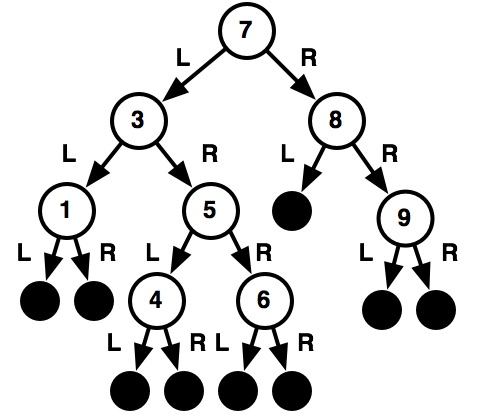
\includegraphics[scale=.75]{binary-search-trees/bst2}~~~~~~~
  \raisebox{.4in}{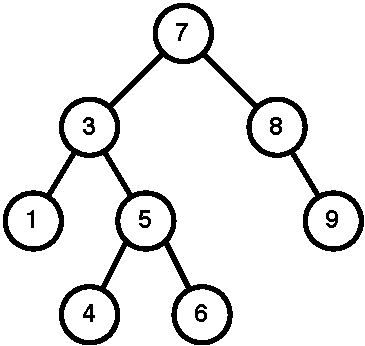
\includegraphics[scale=.75]{binary-search-trees/bst3}}
\end{center}
On the left the $L$ and $R$ indicate the left (first) and right
(second) child, respectively.  All internal nodes (white) have a key
associated with them while the leaves (black) are empty.  The keys
satisfy the BST property---for every node, the keys in the left
subtree are less, and the ones in the right subtree are greater. 


\smallskip 

In the illustration on the left, the edges are oriented away from the
root. They could have also been oriented towards the root.
%
When illustrating binary search trees, we usually replace the directed
arcs with undirected edges, leaving the orientation to be implicit.
%
We also draw the left and right subtrees of a node on its left and
right respectively.
%
Following this convention, we can draw the tree on the left above as
shown an the right.
%
We use this convention in future figures.
\end{example}


\section{The BST Abstract Data Type}
\label{sec:bst::adt}

\newcommand{\bstt}{\tttt}


\adtref{bst::adt} describes an ADT for BSTs parametrized by a totally
ordered key set. We briefly describe this ADT and present some
examples. As we shall see, the BST ADT can be implemented in many
ways.  In order to present concrete examples, we assume an
implementation but do not specify it.


\input{binary-search-trees/fig-adt-spec}

The ADT supports the constructor operations
\cd{empty} and \cd{singleton} for creating an empty BST and BST
with a single key. 
%
The function \cd{find} searches for a given key and returns a
boolean indicating success.
%
\begin{simpleexample}
Searching in BSTs illustrated.

\begin{itemize}
\item 
Searching for  $5$  in the input tree returns \cd{true}.
%
\[
\cd{find}
\left(
\raisebox{-.45in}{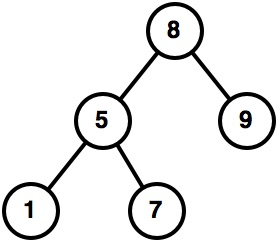
\includegraphics[scale=.6]{binary-search-trees/bst4}}
\right) 
~~5
=
~\cd{true}
\]

\item 
Searching for  $6$  in the input tree returns \cd{false}.
%
\[
\cd{find}
\left(
\raisebox{-.45in}{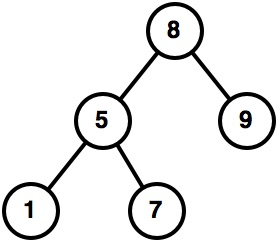
\includegraphics[scale=.6]{binary-search-trees/bst4}}
\right) 
~~6
= \
\cd{false}
\]

\end{itemize}
\end{simpleexample}


%
The functions \cd{insert} and \cd{delete} insert and delete a
given key into or from the BST.
%
\begin{example}
Inserting the key $6$  into the input tree returns a new tree including $6$.
%
\[
\cd{insert}
\left(
\raisebox{-10mm}{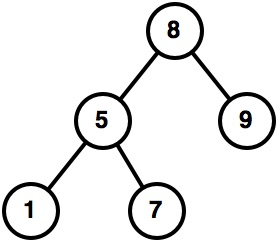
\includegraphics[scale=.6]{binary-search-trees/bst4}}
\right) 
~~6
=
\raisebox{-20mm}{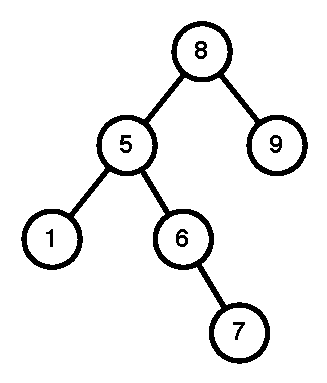
\includegraphics[scale=.6]{binary-search-trees/bst5}}
\]
\end{example}

\begin{example}
Deleting the key  $6$ from the input tree returns a tree without it.
%
\[
\cd{delete}
\left(
\raisebox{-20mm}{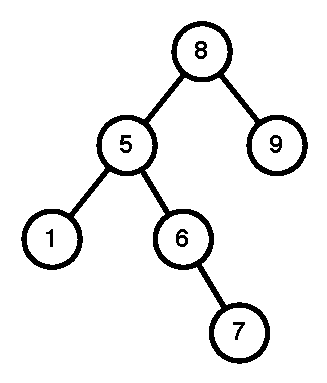
\includegraphics[scale=.6]{binary-search-trees/bst5}}
\right) 
~~6
= 
\raisebox{-10mm}{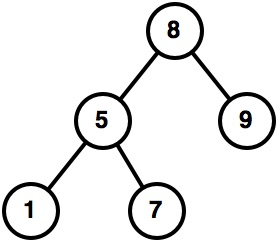
\includegraphics[scale=.6]{binary-search-trees/bst4}}
\]

\end{example}


%
The function \cd{union} takes two BSTs and returns a BST that
contains all the keys in them; \cd{union} is an aggregate insert
operation.
% 
The function \cd{intersection} takes two BSTs and returns a BST
that contains the keys common in both.
% 
The function \cd{difference} takes two BSTs $t_1$ and $t_2$ and returns
a BST that contains the keys in $t_1$ that are not in $t_2$;
\cd{difference} is an aggregate delete operation.

The function \cd{split} takes a tree $t$ and a key $k$ and
splits $t$ into two trees: one consisting of all the keys of $t$ less
than $k$, and another consisting of all the keys of $t$ greater than
$k$.  
%
It also returns a Boolean value indicating whether $k$ appears in $t$.
%
The exact structure of the trees returned by \cd{split} can differ
from one implementation to another: the specification only requires
that the resulting trees to be valid BSTs and that they contain the
keys less than $k$ and greater than $k$, leaving their structure
otherwise unspecified.



\begin{example}

The function \cd{split} illustrated.

\begin{itemize}
\item 
Splitting the input tree at $6$ yields two trees, consisting of the
keys less that $6$ and those greater that $6$, indicating also that
$6$ is not in the input tree. 

\[
\cd{split}
\left(
\raisebox{-.45in}{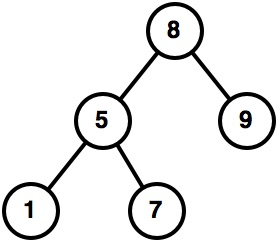
\includegraphics[scale=.6]{binary-search-trees/bst4}}
\right)
~~6
\Rightarrow 
\left(
\raisebox{-.27in}{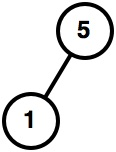
\includegraphics[scale=.6]{binary-search-trees/bst4a}}~~,
~\cd{False}~,~~
\raisebox{-.27in}{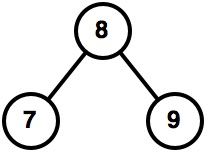
\includegraphics[scale=.6]{binary-search-trees/bst4b}}
\right) 
\]

\item 
Splitting the input tree at $5$ yields two trees, consisting of the
keys less than $5$ and those greater than $5$, indicating also that
$5$ is found in the input tree. 


\[
\cd{split}
\left(
\raisebox{-.45in}{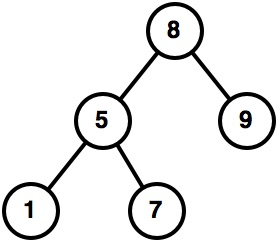
\includegraphics[scale=.6]{binary-search-trees/bst4}}
\right) 
~~5
\Rightarrow 
\left(
\raisebox{-.1in}{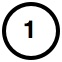
\includegraphics[scale=.6]{binary-search-trees/bst4c}}~~,
~\cd{True}~,~~
\raisebox{-.27in}{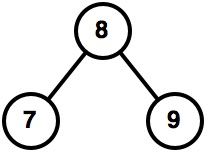
\includegraphics[scale=.6]{binary-search-trees/bst4b}}
\right) 
\]
\end{itemize}
\end{example}

The function \cd{join} takes two trees $t_1$ and $t_2$
such that all the keys in $t_1$ are less than the keys in $t_2$.  The
function returns a tree that contains all the keys in $t_1$ and $t_2$.
%
The exact structure of the tree returned by \cd{join} can differ
from one implementation to another: the specification only requires
that the resulting tree is a valid BST and that it contains all the
keys in the trees joined.



\begin{example}
The function \cd{join} illustrated.

\[
\cd{join}
\left(
\raisebox{-.27in}{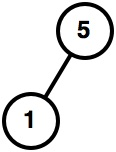
\includegraphics[scale=.6]{binary-search-trees/bst4a}}
\right)
\left(
\raisebox{-.27in}{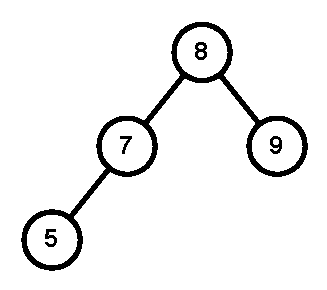
\includegraphics[scale=.6]{binary-search-trees/bst6}}
\right) 
\Rightarrow
\raisebox{-.45in}{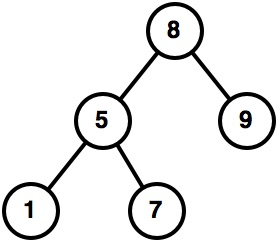
\includegraphics[scale=.6]{binary-search-trees/bst4}}
\]
\end{example}


\section{Implementation via Balancing}
\label{sec:bst::bsts-review}

The main idea behind the implementation of BSTs is to organize the
keys such that
\begin{enumerate}
\item
a specific key can be located by following a branch in the tree,
performing key comparisons along the way, and

\item a set of keys that constitute a contiguous range in a sorted
  order of keys in the tree can be moved as a chunk by performing
  constant work.
\end{enumerate}

To see how we can search in a tree, consider searching for a key $k$
in a tree $t$ whose root is $r$.
%
We can start at the root $r$ and if $k$ equals the key at the root,
$k(r)$, then we have found our key, otherwise if $k < k(r)$, then we
know that $k$ cannot appear in the right subtree, so we only need to
search the left subtree, and if $k > k(r)$, then we only have to
search the right subtree.  Continuing the search, we will either find
the key or reach a leaf and conclude that the key is not in the tree.
%
In both cases we have followed a single path through the BST starting
at the root.

\begin{example}

A successful search for $7$ and an unsuccessful search for $4$ in the
given tree.  Search paths are highlighted.


\begin{center}
\parbox[t]{3cm}
{
\vspace*{0cm}
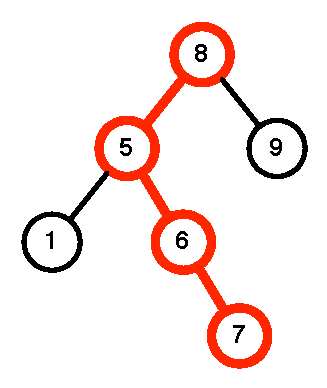
\includegraphics[width=3cm]{binary-search-trees/bst5-search-7}\
}
%
\hspace*{3cm}
%
\parbox[t]{3cm}
{
\vspace*{0cm}
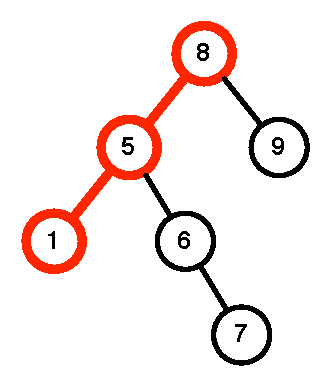
\includegraphics[width=3cm]{binary-search-trees/bst5-search-4}
}
\end{center}
\end{example}

To see how we can operate on a range of keys, note first that each
subtree in a binary tree contains all the keys that are within a
specific range. 
%
We can find such a range by performing a search as
described---in fact, a search as described identifies a possibly empty
range. Once we find a range of keys, we can operate on them as a group
by handling their root.
%
For example, we can move the whole subtree to another location by
linking the root to another parent.

\begin{example}
Consider the tree shows below on the left, we can handle all the keys
that are less than $8$ by holding the subtree rooted at $5$, the left
child of $8$.  For example, we can make $5$ the left child of $9$ and
delete $8$ from the tree. Note that if $8$ remains in the tree, the
resulting tree would not be a valid BST.

\begin{center}
\parbox[t]{3cm}
{
\vspace*{0cm}
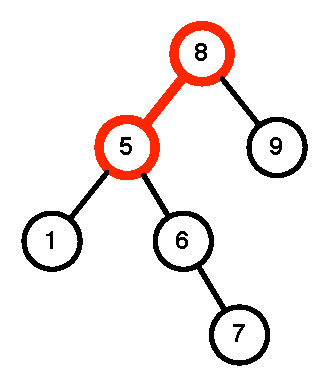
\includegraphics[width=3cm]{binary-search-trees/bst5-search-5}
}
\hspace*{3cm}
\parbox[t]{3cm}
{
\vspace*{0cm}
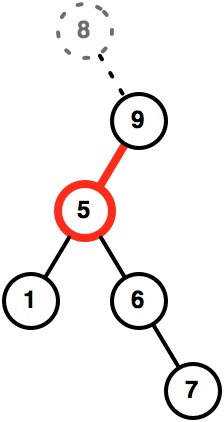
\includegraphics[width=2.5cm]{binary-search-trees/bst5-move-5}
}
\end{center}
\end{example}

%%%% Commented out because trees, leaf, inode etc undefined
%% We can write the algorithm for finding a key in a BST as
%% follows.

%% \begin{algorithm}[Finding a key in a BST]~
%% \begin{lstlisting}[numbers=none]
%% fun find$(T,k)$ =
%%   case $T$ of 
%%      Leaf => False
%%    | iNode$(L,k',R)$ => 
%%        case compare$(k,k')$ of
%%           Less => find$(L,k)$
%%         | Equal => true
%%         | Greater => find$(R,k)$
%% \end{lstlisting}
%% \end{algorithm}

%% We note that, while we don't consider this in this \bc, this form of
%% search in a BST can be generalized beyond binary trees to work with
%% tree nodes with higher degrees.  To do this, for a node with $k$
%% children, we would need $k-1$ keys so separate each of the children.
%% In this book we only cover binary search trees.

By finding a range of keys by traversing a path in the BST, and by
moving ranges with constant work, it turns out to be possible to
implement all the operations in the BST ADT efficiently as long as the
paths traversed are not too long.
%
One way to guarantee absence of long paths is to make sure that the
tree remains balanced, i.e., the longest paths have approximately
the same length.
%
A binary tree is defined to be \defn{perfectly balanced} if it has the
minimum possible height.  
%
For a binary search tree with $n$ keys, a perfectly balanced tree has
height exactly $\lceil \lg (n + 1) \rceil$.

Ideally we would like to use only perfectly balanced trees.  
%
If we never make changes to the tree, we could balance it
once and for all.
%
If, however, we want to update the tree by, for example, inserting new
keys, then maintaining such perfect balance is costly.  
%
In fact, it turns out to be impossible to maintain a perfectly
balanced tree while allowing insertions in $O(\lg n)$ work.  
%
BST data structures therefore aim to keep approximate balance instead
of a perfect one.  We refer to a BST data structure as {\em nearly
  balanced} or simply as {\em balanced} if all trees with $n$ elements
have height $O(\lg n)$, perhaps in expectation or with high
probability.

There are many balanced BST data structures.  Most either try to
maintain height balance (the children of a node are about the same
height) or weight balance (the children of a node are about the same
size).  Here we list a few such data structures:

\begin{enumerate}
\item \defn{AVL trees} are the earliest nearly balanced BST data
  structure (1962).  It maintains the invariant that the two children
  of each node differ in height by at most one, which in turn implies
  approximate balance.

\item \defn{Red-Black trees} maintain the invariant that all leaves
  have a depth that is within a factor of 2 of each other.  The depth
  invariant is ensured by a scheme of coloring the nodes red and
  black.

\item \defn{Weight balanced (BB[$\alpha$]) trees} maintain the
  invariant that the left and right subtrees of a node of size $n$
  each have size at least $\alpha n$ for $0 < \alpha \leq
  1 - \frac{1}{\sqrt{2}}$.  The BB stands for bounded balance, and adjusting
  $\alpha$ gives a tradeoff between search and update costs.

\item \defn{Treaps} associate a random priority with every key and
  maintain the invariant that the keys are stored in heap order with
  respect to their priorities (the term ``Treap'' is short for ``tree
  heap'').  Treaps guarantee approximate balance with
  high-probability.

\item \defn{Splay trees} are an amortized data structure that does not
  guarantee approximate balance, but instead guarantees that for any sequence
  of $m$ insert, find and delete operations each does $O(\lg n)$
  amortized work.
\end{enumerate}
There are dozens of other balanced BST data structures (e.g. scapegoat
trees and skip lists), as well as many that allow larger degrees,
including 2--3 trees, brother trees, and B trees.  
%
In this chapter we will cover Treaps.

%, red-black trees, and briefly AVL trees.

\begin{todo}

Bob Harper comment:
misleading discussion? pages 226-227 the discussion of splay trees,
etc ignores the important issue of single-threaded vs multi-threaded
data structures; amortization doesn't work for the multithreaded case.
do the treaps work for that case?

It might indeed be worthwhile to discuss the weakness of amortization
with respect to persistence.  Though this seems a bit advanced for
this material.  Further thought is needed...

\end{todo}


\section{A Parametric Implementation}
\label{sec:bst::parametric}

We describe a minimalist implementation of the BST ADT based on two
functions, \cd{split} and \cd{join}. 
%
Since the implementation depends on just these two functions, we refer
to it as a parametric implementation.
%
\dsref{bst::parametric} illustrates the parametric implementation,
assuming that the implementation of \cd{split} and \cd{join} are
supplied. 
%
The implementation defines the tree type as consisting of
leaves or internal nodes with left and right subtrees and a key.
%
The auxiliary function, \cd{joinM} takes two trees $t_1$ and $t_2$
and a ``middle'' key $k$ that is sandwiched between the two
trees---that is $k$ is greater than all the keys in $t_1$ and less
than all the keys in $t_2$---and returns a tree that contains all the
keys in $t_1$ and $t_2$ as well as $k$.

\begin{datastructure}[Implementing the BST ADT with \cd{split} and \cd{join}]
\label{ds:bst::parametric}
\begin{lstlisting}
type $\tttt$ = Leaf | Node of ($\tttt$ ** $\kkk$ ** $\tttt$)
split $t$ $k$ = ... (* as given *)
join $t_1$ $t_2$ = ... (* as given *)

joinM $t_1$ $k$ $t_2$ = join $t_1$ (join (singleton $k$) $t_2$)
empty = Leaf
singleton $(k)$ = Node(Leaf,$k$,Leaf)  
find $t$ $k$ = let (_,$v$,_) = split $t$ $k$  in $v$ end 
delete $t$ $k$ = let $(l,\_,r)$ = split $t$ $k$ in join $l$ $r$ end
insert $t$ $k$ = let $(l,\_,r)$ = split $t$ $k$ in joinM $l$ $k$ $r$ end 

intersect $t_1$ $t_2$ =
  case ($t_1$,$t_2$) 
  | (Leaf,_) => Leaf
  | (_,Leaf) => Leaf
  | (Node $(l_1,k_1,r_1)$,_) => 
    let $(l_2,b,r_2)$ = split $t_2$ $k_1$
       $(l,r)$ = (intersect $l_1$ $l_2$) || (intersect $r_1$ $r_2$)
    in if $b$ then joinM $l$ $k_1$ $r$ else join $l$ $r$ end

difference $t_1$ $t_2$ =
  case ($t_1$, $t_2$)
  | (Leaf,_) => Leaf
  | (_,Leaf) => $t_1$
  | (Node $(l_1,k_1,r_1)$,_) => 
    let $(l_2,b,r_2)$ = split $t_2$ $k_1$
        $(l,r)$ = (difference $l_1$ $l_2$) || (difference $r_1$ $r_2$)
    in if $b$ then join $l$ $r$ else joinM $L$ $k_1$ $r$ end

union $t_1$ $t_2$ =
  case ($t_1$,$t_2$)
  | (Leaf,_) => $t_2$
  | (_,Leaf) => $t_1$
  | (Node $(l_1,k_1,r_1)$,_) =>   
    let $(l_2,\_,r_2)$ = split $t_2$ $k_1$
        $(l,r)$ = (union $l_1$ $l_2$) || (union $r_1$ $r_2$)
    in joinM $l$ $k_1$ $r$ end    
\end{lstlisting}
\end{datastructure}



The function \cd{find} is easily implementable with a
\cd{split}, which indicates whether the key used for splitting is
found in the tree or not.
%
To implement \cd{insert} of a key $k$ into a tree, we first
\cd{split} the tree at $k$ and then join the two returned
trees along with key $k$ using \cd{joinM}.
%
To implement \cd{delete} of a key $k$ from a tree, we first
\cd{split} the tree at $k$ and then join the two returned
trees with \cd{join}. 
%
If the key $k$ was found, this gives us a tree that does not contain
the $k$; otherwise we obtain a tree of the same set of keys (though
the structure of the tree may be different internally depending on the
implementation of \cd{split} and \cd{join}).

The implementation of \cd{union} uses divide and conquer.  The idea is
to split both trees at some key $k$, recursively union the two parts
with keys less than $k$, and the two parts with keys greater than $k$
and then join them.  
%
There are different ways to select the key $k$ used to split the tree.
%
One way is to use the key at the root of one of the two trees, for
example the first tree, and split the second tree with it; this is the
approach take in the parametric implementation.



\begin{example}
The union of tree $t_1$ and $t_2$ illustrated.

\begin{center}
  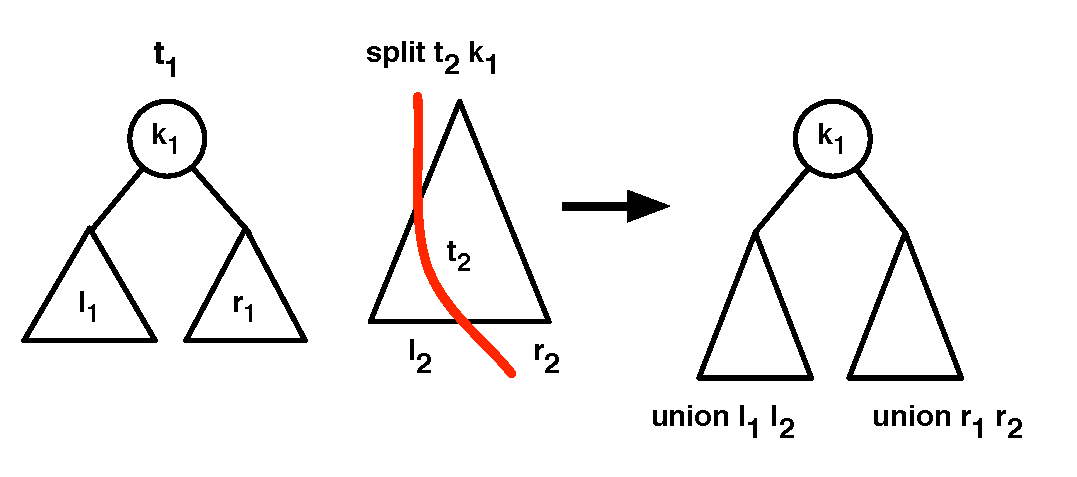
\includegraphics[scale=.7]{binary-search-trees/union-dia1}
\end{center}
\label{example:tree-union}
\end{example}

%For simplicity, this
%version returns the value from $t_1$ if a key appears in both BSTs,

The implementation of \cd{intersection} uses a divide-and-conquer
approach similar to that  of \cd{union}.  
%
As in \cd{union}, we split both trees by using the key $k_1$ at the
root of the first tree, and compute intersections recursively.
%
We then compute the result by joining the results from the recursive
calls and including the key $k_1$ if it is found in both trees.
%
\begin{question}
How does the implementation accounts for all possible shared keys when
we divide the input trees into two and calculate intersections
recursively?  What if a key on the left matches a key on the right
half of the other tree?
\end{question}
%
Note that since the trees are BSTs, checking for the intersections of
left and right subtrees recursively and is guaranteed to find all
shared keys because the \cd{split} operation places all keys less
than and greater than the given key to two separate trees.

\begin{exercise}
  Prove correct the functions \cd{intersection}, \cd{difference}, and
  \cd{union}.
\end{exercise}

\section{Cost Specification}
\label{sec:bst::cost}

There are many ways to implement an efficient data structure that
matches our BST ADT, many of these implementation more or less match
the same cost specification, with the main difference being whether
the bounds are worst-case, expected case (probabilistic), or
amortized.  
%
These implementations all use balancing techniques to ensure that the
depth of the BST remains $O(\lg{n})$, where $n$ is the number of keys
in the tree.  
%
For the purposes specifying the costs, we don't distinguish between
worst-case, amortized, and probabilistic bounds, because we can always
rely on the existence of an implementation that matches the desired
cost specification.  
%
When using specific data structures that match the specified bounds in
an amortized or randomized sense, we will try to be careful when
specifying the bounds.


\input{binary-search-trees/fig-bst-cost}

\costref{bst::costs} shows the costs for the BST ADT as can be
realized by several balanced BST data structures such as Treaps (in
expectation), red-black trees (in the worst case), and splay trees
(amortized). As may be expected the cost of \cd{empty} and
\cd{singleton} are constant.
%

For the rest of the operations, we justify the cost bounds by assuming
the existence of logarithmic time \cd{split} and \cd{join} operations,
and by using our parametric implementation described above.
%
The work and span costs of \cd{find}, \cd{insert}, and
\cd{delete} are determined by the \cd{split} and \cd{join}
operation and are thus logarithmic in the size of the tree.
%

The cost bounds on \cd{union}, \cd{intersection}, and
\cd{difference}, which are similar are more difficult to see.  Let's
analyze the cost for \cd{union} as implemented by the parametric
implementation. It is easy to apply a similar analysis to
\cd{intersection} and \cd{difference}.

Consider now a call to \cd{union} with parameters
$t_1$ and $t_2$.  To simplify the analysis, we will make the following
assumptions:
\begin{enumerate}
\item $t_1$ is perfectly balanced (i.e., the left and right subtrees of
  the root have size at most $|t_1|/2$), 
\item each time a key from $t_1$ splits $t_2$, it splits the tree in
  exactly in half, and
\item $|t_1| < |t_2|$.
\end{enumerate}
Later we will relax these assumptions.  Let us define $m = |t_1|$ and
$n = |t_2|$ (recall the size of a tree is the number of keys in it).
With these assumptions and examining the algorithm we can then write
the following recurrence for the work of \cd{union}:
\begin{align*}
  W_{\mbox{union}}(m, n) &\leq 2W_{\mbox{union}}(m/2,n/2) + W_{\mbox{split}}(n)
+ W_{\mbox{join}}(n+m) + O(1)\\
   & \leq  2W_{\mbox{union}}(m/2, n/2) + O(\lg n)~.
\end{align*}  
The size for join is the sum of the two sizes, $m+n$, but since 
$m \leq n$, $O(\lg (n + m))$ is equivalent to $O(\lg n)$.
We also have the base case
\begin{align*}
  W_{\mbox{union}}(1, n) & \leq 2W_{\mbox{union}}(0,n/2) + W_{\mbox{split}}(n)
+ W_{\mbox{join}}(n) + O(1)\\
         & \leq O(\lg n)~.
\end{align*}
The final inequality holds because $2W_{\mbox{union}}(0,n) = O(1)$.

We can draw the recursion tree showing the work performed by the
splitting of $t_2$ and by the joining of the results as follows.  For
simplicity of the argument, let's assume that the leaves of the tree
correspond to the case for $m = 1$.

%This figure should be changed so "n" is replaced by "N" except the
%bottom level should be "each costs log (1 + n/m)"

\begin{center}
  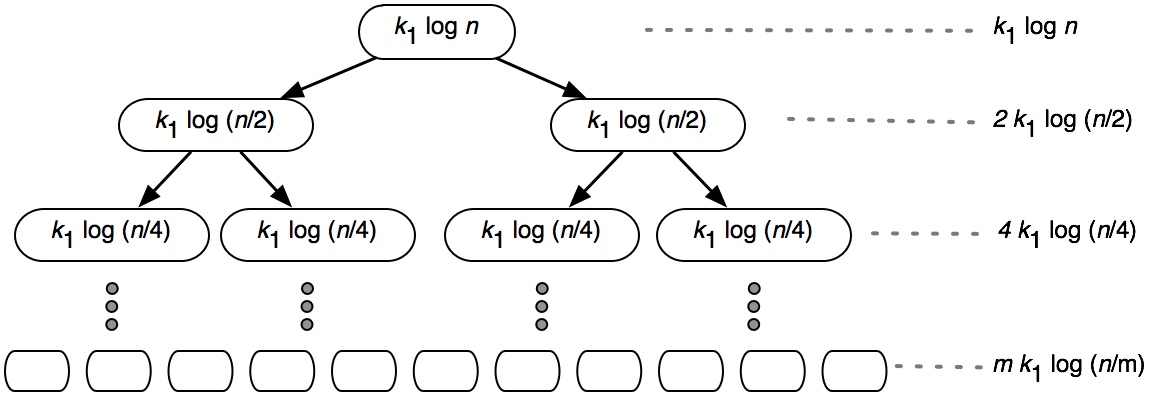
\includegraphics[scale=.65]{binary-search-trees/recurtree2}
\end{center}
%

\paragraph{Brick method.}
Let's analyze the structure of the recursion tree shown above.
%
\begin{question}
How many leaves are there?
\end{question}
%
We can find the number of leaves in the tree by examining the work
recurrence.  Notice that in the recurrence, the tree bottoms out when
$m = 1$ and before that, $m$ always gets split in half (remember that
$t_1$ is perfectly balanced).  The tree $t_2$ does not affects the
shape of the recursion tree or the stopping condition. Thus, there are
exactly $m$ leaves in the tree.  
%
In fact, the recursion can be rewritten as a recursion of the form
$W(m) = 2W(m/2) + \ldots $, which means that there are $m$ leaves.
%
\begin{question}
How deep are the leaves?
\end{question}
%
By the same reasoning, we can see that the leaves are $(1 + \lg m)$
deep.

Let's now determine the size of $t_2$ at the leaves.  
%
We have $m$ keys in $t_1$ to start with, and they split $t_2$ evenly
all the way down to the level of the leaves (by assumption). Thus, the
leaves have all the same size of $\frac{n}{m}$.
%
Therefore, each leaf adds a $O(\lg (1+\frac{n}{m}))$ term to the work
(the $1+$ is needed to deal with the case that $n = m$).  Since there
are $m$ leaves, the whole bottom level costs $O(m \lg (1+
\frac{n}{m}))$.  

We will now prove that the cost at the bottom level is indeed
asymptotically the same as the total work.  In other words, the tree
is leaves-dominated.  It is possible to prove that the tree is
leaves-dominated by computing the ratio of the work at adjacent
levels, i.e., the ratio $\frac{2^{i-1}  \lg{n/2^{i-1}}}{2^i 
  \lg{n/2^{i}}} = \frac{1}{2} \frac{\lg{n} - i + 1 }{\lg{n} - i}$,
where $i \le \lg{m} < \lg{n}$. This ratio is less than $1$ for all
levels except for the last level, where by taking $i = \lg{n} - 1$ we
have
\[
 \frac{1}{2} \frac{\lg{n} - i +1 }{\lg{n} - i}
 \le
 \frac{1}{2} \frac{1}{\lg{n} - \lg{n} +1 + 1}{\lg{n} - \lg{n}+1}
= \frac{1}{1}.
\]
Thus the total work is asymptotically dominated by the total work of
the leaves, which is $\bigoh{m\lg{n/m}}$.


\paragraph{Direct derivation.}
We can establish the same fact more precisely.  Let's start by writing
the total cost by summing over all levels, omitting for simplicity the
constant factors, and assuming that $n = 2^a$ and $m = 2^b$,
\[
W(n,m) = \sum_{i = 0}^{b}{2^i \lg{\frac{n}{2^i}}}.
\]
We can rewrite this sum as 
\[
\sum_{i = 0}^{b}{2^i \lg{\frac{n}{2^i}}} = 
\lg{n}\sum_{i = 0}^{b}{2^i} - \sum_{i = 0}^{b}{i\,2^i}.
= a\sum_{i = 0}^{b}{2^i} - \sum_{i = 0}^{b}{i\,2^i}.
\]
Let's now focus on the second term. Note that 
\[
\sum_{i = 0}^{b}{i\,2^i} 
=
\sum_{i = 0}^{b}{\sum_{j=i}^{b}2^j} 
=
\sum_{i = 0}^{b}{\left(\sum_{j=0}^{b}{2^j} - \sum_{k=0}^{i-1}2^k\right). }
\]
Substituting the closed form for each inner summation and simplifying
leads to
\[
\begin{array}{ll}
= & \sum_{i = 0}^{b}{\left( (2^{b+1}-1) - (2^{i}-1) \right)}.
\\[2mm]
= &  (b+1) (2^{b+1}-1) - \sum_{i = 0}^{b}{(2^{i}-1)}
\\[2mm]
= &  (b+1) (2^{b+1}-1) - \left( 2^{b+1}-1 - (b+1) \right)
\\[2mm]
= &  (b+1) (2^{b+1}-1) - \left( 2^{b+1}-1 - (b+1) \right)
\\[2mm]
= &  b\,2^{b+1} + 1.
\end{array}
\]

Let's now go back and plug this into the original work bound and simplify
\[
\begin{array}{lll}
W(n,m) & = &\sum_{i = 0}^{b}{2^i \lg{\frac{n}{2^i}}}
\\[2mm]
& = & a\sum_{i = 0}^{b}{2^i} - \sum_{i = 0}^{b}{i\,2^i}
\\[2mm]
& = & a\,(2^{b+1}-1) -  (b\,2^{b+1} + 1)
\\[2mm]
& = & a\,2^{b+1}-a - b\,2^{b+1} -1
%\\
= 2m (a-b) - a -1
\\[2mm]
& = & 2m (\lg{n}-\lg{m}) - a -1
%\\
= 2m \lg{\frac{n}{m}} - a -1
\\[2mm]
& = & \bigoh{m \, \lg{\frac{n}{m}}}.
\end{array}
\]

While the direct method may seem complicated, it is more robust than
the brick method, because it can be applied to analyze essentially any
algorithm, whereas the Brick method requires establishing a geometric
relationship between the cost terms at the levels of the tree.
%

\paragraph{Removing the Assumptions.}

Of course, in reality, our keys in $t_1$ won't split subtrees of $t_2$
in half every time.  But it turns out that any unevenness in the
splitting only helps reduce the work---i.e., the perfect split is the
worst case.  We won't go through a rigorous argument, but if we keep
the assumption that $t_1$ is perfectly balanced, then the shape of the
recursion tree stays the same.  What is now different is the cost at
each level.  Let us try to analyze the cost at level~$i$.  At this
level, there are $k = 2^i$ nodes in the recursion tree. Say the sizes
of $t_2$ at these nodes are $n_1, \dots, n_k$, where $\sum_j n_j =
n$. Then, the total cost for this level is
\[
c \cdot \sum_{j=1}^k \lg (n_j) \;\;\leq\;\; c \cdot \sum_{j=1}^k \lg (n/k) =
c\cdot 2^i \cdot \lg (n/2^i),
\]
where we used the fact that the logarithm function is
concave\footnote{This is also known as Jensen's inequality.}.  Thus,
the tree remains leaf-dominated and the same reasoning shows that the
total work is $O(m \lg (1 + \frac{n}{m}))$.

Still, in reality, $t_1$ doesn't have to be perfectly balanced as we
assumed. To generalize the analysis, we just need a tree with
$O(\lg{m})$ height.  Thus, we only need $t_1$ to be approximately
balanced. 

Finally, we assumed that $t_1$ is larger that $t_2$.  If it is
smaller, then we can reverse the order of arguments, so in this case,
there is no loss of generality.  If they are the same size, we need to
be a bit more precise in our handling of the base case in our
summation but this is all.

We end by remarking that as described, the span of \cunion{} is
$O(\lg^2 n)$, but this can be improved to $O(\lg n)$ by changing the
algorithm slightly.

In summary, \cunion{} can be implemented in $O(m \lg (1 +
\tfrac{n}m))$ work and span $O(\lg n)$.  

Essentially the same analysis applies to the functions
\cd{intersection} and \cd{difference}, whose structures are the same
as \cd{union}, except for an additional constant work and span for
the conditional (\cd{if}) expression.
 
\section{Treaps}
\label{sec:bst::treaps}

Our parametric implementation established an interesting fact: to
implement the BST ADT efficiently, we only need to provide efficient
\cd{split} and \cd{join} operations.  In this section, we
present a data structure called {\em Treaps} that can support
\cd{split} and \cd{join} operations in expected logarithmic work
and span.
%
Treaps achieve their efficiency by maintaining BSTs that are
probabilistically balanced. Of the many balanced BST data structures,
Treaps are likely the simplest, but, since they are randomized, they
only guarantee approximate balance with high probability.

\begin{notesonly}

  To see the idea behind Treaps, let's first discuss how we can map a
  sequence of keys to a BST. Given $S$, a sequence of unique keys,
  let's start with an empty BST and insert the keys in $S$ into the
  BST one by one starting from left to right.  To insert a key $k$, we
  perform a search for $k$ in the current BST and let $u$ be the leaf
  where the (unsuccessful) search terminates.  To insert $k$ into the
  tree, we replace $u$ with a new node with key $k$.

\begin{simpleexample}

We can map the sequence $\cseq{8,9,5,6,1,7}$ to a BST by inserting the keys from
left to right.

\begin{center}
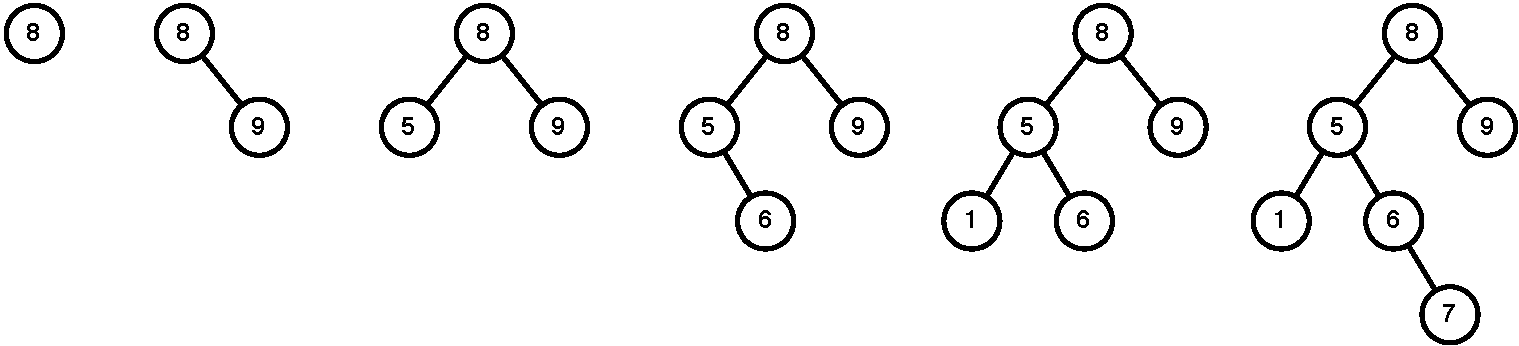
\includegraphics[width=14cm]{binary-search-trees/bst5-build}
\end{center}

\end{simpleexample}

\begin{question}
What can we say about the height of such a tree? 
\end{question}
Note now that the height of the BST will be directly determined by the
input sequence.  Specifically, the specific order---or
permutation---in which the keys are inserted will determine the
height.  For most permutations, the tree will be reasonably well
balanced because we get an unbalanced tree only in cases where an
element partitions the following keys unevenly.  Since we have
many more even partitions for a given set of keys (many ``middle''
keys), many permutations create balanced trees.

\begin{question}
Can we take advantage of this observation somehow? 
\end{question}
%
Recall that the BST ADT does not care about the specific structure of
the BST but only the set of keys in the tree. We can take advantage of
this observation by selecting a (uniformly) random permutation of the keys and
constructing the BST based on this permutation.  Since most
permutations give us reasonably balanced trees, this approach should
give us a balanced tree.


\begin{question}
Suppose that we were given the keys in the sequence one by one instead
of all at once.  Can you think of a way to select a uniformly random
permutation?
\end{question}

Observe now that we can select a uniformly random permutation even if
we don't have all the keys by assigning a random priority to each key
as it arrives and building our BST by considering the keys in the
priority order.  By assigning priorities randomly, we essentially
guarantee that we always build our tree on a uniformly randomly
selected permutation.
%
This is one of the main ideas behind Treaps: Treaps can be viewed as
maintaining a BST on a uniformly random permutation of the keys in the
tree. To achieve this ``imitation of randomly ordered insertions''
we associate a priority with each key and require the BST to be ``heap
ordered'' with respect to priorities.
\end{notesonly}

The idea behind Treaps is to associate a uniformly randomly selected
priority to each key and maintain a priority order between keys in
addition to the binary-search-tree order.  The priority order between
keys resemble the order used in binary heaps, leading to the name
``Tree Heap'' or ``Treap.'' We define Treaps as follows.
%
\begin{definition}[Treap]
  A Treap is a binary search tree over a set $K$ along with a
  \defn{priority} for each key given by \[p : \kkk \rightarrow
  \tyint~,\] that in addition to satisfying the BST property on the
  keys $K$, satisfies the heap property on the priorities $p(k), k \in
  K$, i.e., for every internal node $v$ with left and right children
  $u$ and $w$:
\[
p(k(v)) \geq p(k(u)) \mbox{ and } p(k(v)) \geq p(k(w)),
\]
where $k(v)$ denotes the key of a node.
\end{definition}

\begin{example}
The following key-priority pairs $(k,p(k))$,
\[ (a,3), (b,9), (c, 2), (e,6), (f, 5)~,\] where the keys are ordered
alphabetically, form the following Treap:
\begin{center}
  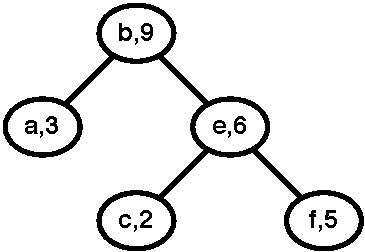
\includegraphics[width=1.5in]{binary-search-trees/treap-examp}
\end{center}
since $9$ is larger than $3$ and $6$, and $6$ is larger than $2$ and
$5$.
\end{example}
\begin{exercise}
Prove that if the priorities are unique, then there is exactly one tree
structure that satisfies the Treap properties.
\end{exercise}

So how do we assign priorities?  As we briefly suggested in the
informal discussion above, it turns out that if the priorities are
selected uniformly randomly then the tree is guaranteed to be near
balanced, i.e. $O(\lg |S|)$ height, with high probability.  We will
show this shortly.

\begin{question}
How can we maintain the heap order as we modify the tree?
\end{question}

The second idea behind Treaps is to update the tree structure
according to new priorities efficiently by performing local
reorganizations.
%
Based on our parametrized implementation, we can give an
implementation for the BST ADT with Treaps simply by implementing the
\cd{split} and \cd{join} functions.  \dsref{bst::treaps} shows
such an implementation.  For the implementation we assume, without
loss of generality, that the priorities are integers.  We present only
the code for \cd{split} and \cd{join}; the rest of the
implementation is essentially the same as in \dsref{bst::parametric}
with the only exception that since the nodes now carry priorities, we
will need to account for them as we pattern match on nodes and create
new ones.  In implementing the rest of the functions, there is no
interesting operations on priorities: they simply follow the key that
they belong to.


% We also give a direct implementation of \cd{insert}.

\begin{figure}
\begin{datastructure}[Implementing \adt{BST} with Treaps]~
\label{ds:bst::treaps}
\begin{lstlisting}
type $\tttt$ = Leaf | Node of ($\tttt$ ** $\kkk$ ** $\tyint$ ** $\tttt$)

let empty = Leaf

singleton $k$ = Node(Leaf,$k$,randomInt(),Leaf)

split $t$ $k$ = 
  case $t$ 
  | Leaf => (Leaf, False, Leaf)
  | Node $(l,k',p',r)$ =
      case compare $(k,k')$
      | LESS => @\label{line:bst::treaps::split-less}@
          let $(l',x,r')$ = split $l$ $k$
          in $(l',x,\cdm{Node}(r',k',p',r))$ end @\label{line:bst::treaps::splitnode1}@
      | EQUAL => $($$l$,true,$r$$)$
      | GREATER => @\label{line:bst::treaps::split-greater}@
          let $(l',x,r')$ = split $r$ $k$
          in (Node $(l,k',p',l'),x,r'$) end @\label{line:bst::treaps::splitnode2}@

join $t_1$ $t_2$ =
  case $(t_1,t_2)$
  | (Leaf, _) => $t_2$
  | (_ , Leaf) => $t_1$
  | (Node $(l_1,k_1,p_1,r_1)$, Node $(l_2,k_2,p_2,r_2)$) =>
      if ($p_1 > p_2$) then  @\label{line:bst::treaps::cpri}@
        Node ($l_1$,$k_1$,$p_1$, join $r_1$ $t_2$)
      else
        Node (join $t_1$ $l_2$, $k_2$,$p_2$,$r_2$)
end
\end{lstlisting}
\end{datastructure}
\end{figure}

To implement the function \cd{singleton}, we rely on a function
\cd{randomInt}, which when called returns a (pseudo-)random number.
Such functions are broadly provided by programming languages.

The \cd{split} algorithm recursively traverses the tree from the
root to the key $k$ splitting along the path, and then when returning
from the recursive calls, it puts the subtrees back together.  When
putting back the trees along the path being split through, the
function does not have to compare priorities because $\cd{Node}$ on
\linereftwo{bst::treaps::splitnode1}{bst::treaps::splitnode2},
the priority $p'$ is the highest priority in the input tree $T$ and is
therefore larger than the priorities of either of the subtrees on the
left and right.  Hence \cd{split} maintains the heap property of
treaps.

\begin{example}
A \cd{split} operation on a Treap and key~$c$, which is not in the
Treap.  The \cd{split} traverses the path $\cseq{a,e,b,d}$ turning
right at $a$ and $b$ (\lineref{bst::treaps::split-greater} of the Data
Structure~\ref{ds:bst::treaps}) and turning left at $e$ and $d$
(\lineref{bst::treaps::split-less}).  The pieces are put back together into the two
resulting trees on the way back up the recursion.
\begin{center}
  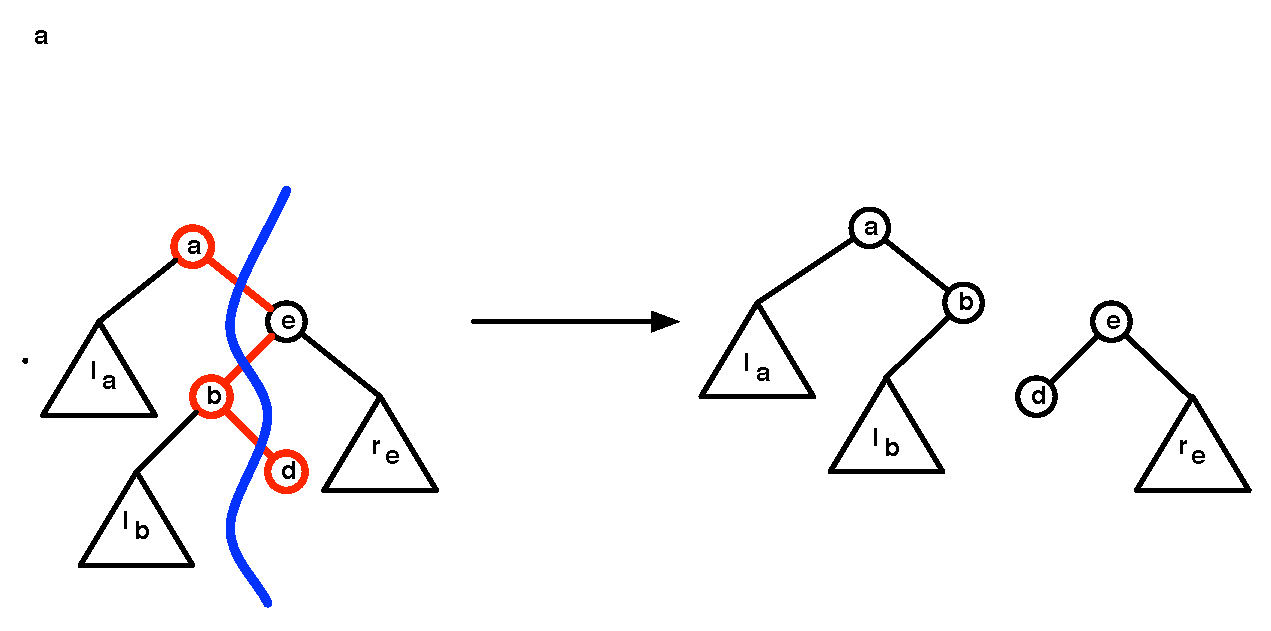
\includegraphics[width=5.7in]{binary-search-trees/bstsplit}
\end{center}
%The actual way the trees will be put back together will depend on the
%balancing scheme.
\end{example}

Unlike the implementation of \cd{split}, the implementation of
\cd{join}$(L,R)$ operates on priorities in order to ensure that the
resulting Treap satisfies the heap priority of Treaps.  Specifically,
given two trees, \cd{join} first compares the priorities of the two
roots, making the larger priority the new root. It then recursively
joins the Treaps consisting of the other tree and the appropriate side
of the new root.  This is illustrated in the following example:
\begin{example}
\label{ex:bst::treap-join}
An illustration of \cd{join}$t_1$ $t_2$ on Treaps.  
%
If $p(k_1) > p(k_2)$, then the function recurs with
$\cd{join}(R_1,t_2)$ and the result becomes the right child of
$k_1$.
\begin{center}
  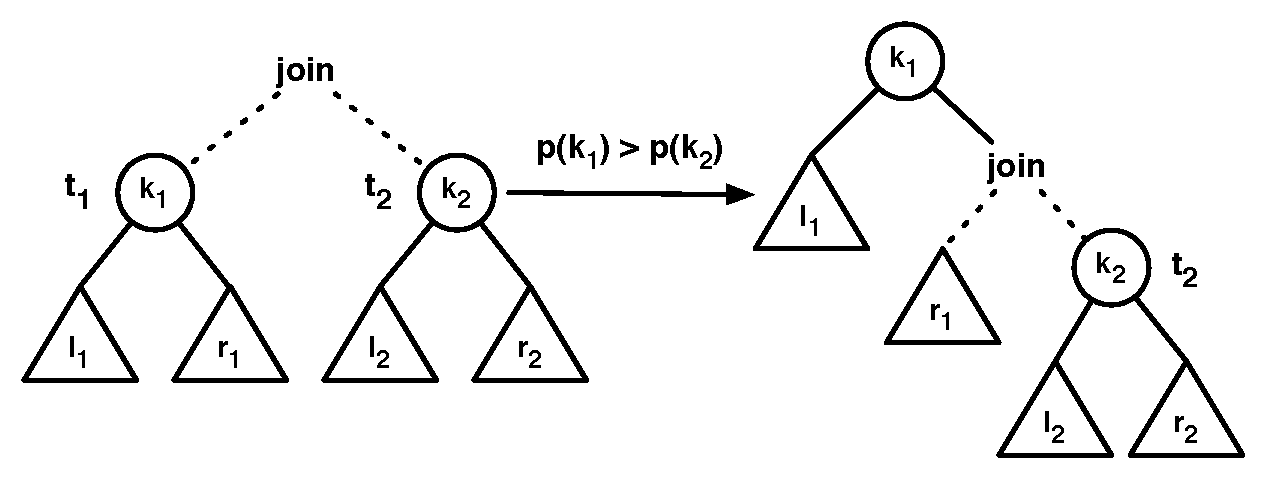
\includegraphics[scale=.6]{binary-search-trees/treap-join}
\end{center}
\end{example}

The path from the root to the leftmost node in a BST is called the
\defn{left spine}, and the path from the root to the rightmost node is
called the \defn{right spine}.  The function $\cd{join}~t_1~t_2$
merges the right spine of $t_1$ with the left spine of $t_2$ based on
the priority order.  This ensures that the priorities are in
decreasing order down the path.
\begin{example}
  An illustration of \cd{join} for Treaps applied to $t_1$ and $t_2$ in
  more detail.  The right spine of $t_1$ consisting of $(b,9)$,
  $(d,6)$ and $(e,5)$ is merged by priority with the left spine of
  $t_2$ consisting of $(h,8)$ and $(g,4)$.  Note that splitting the
  result with the key $f$ will return the original two trees.
\begin{center}
  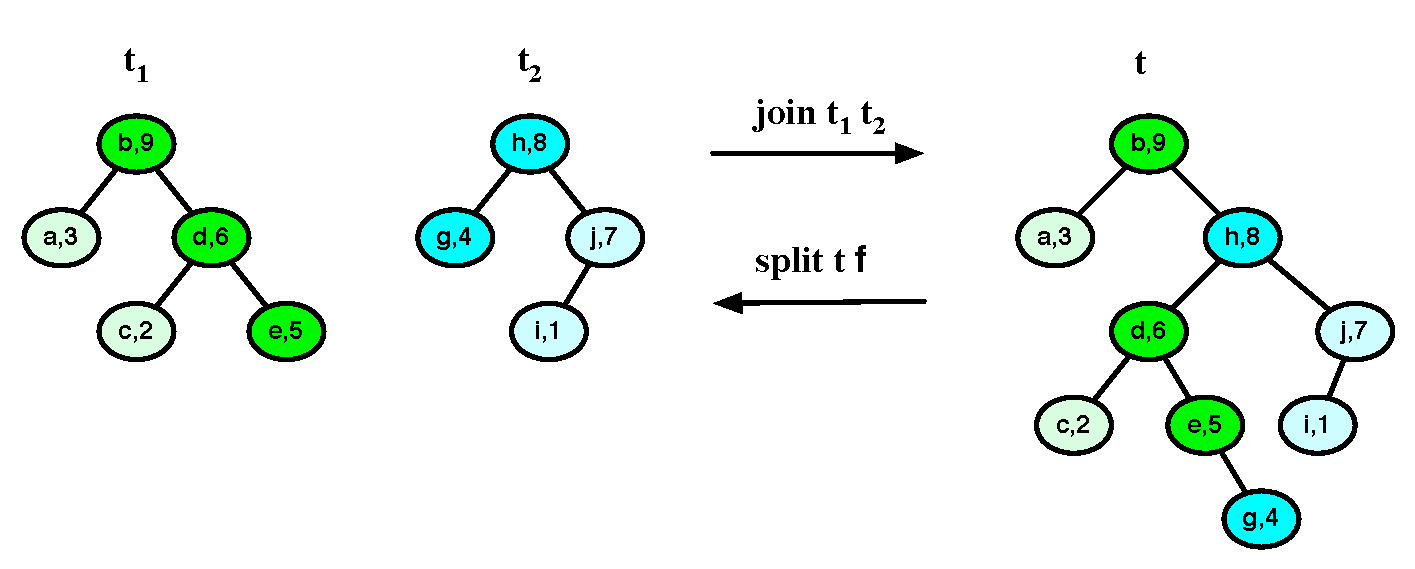
\includegraphics[width=5.8in]{binary-search-trees/treap-examp-join}
\end{center}
\end{example}


%% \begin{figure}
%% \begin{algorithm}[Insertion into a Treap]~
%% \label{alg:treapJoin}
%% \begin{lstlisting}
%% function rotateRight$(\cd{Node}(L_l,k,L_r),k',R)$ =
%%   if $(k > k')$ then Node$(L_l,k,\cd{Node}(L_r,k',R))$  % rotate right
%%   else Node$(\cd{Node}(L_l,k,L_r),k',R)$           % leave as is@\vspace{.1in}@
%% function insert$(T,k)$ =
%%    case $T$ of
%%      Leaf => singleton$(k)$
%%    | Node$(L,k',R)$ => 
%%        case compare$(k,k')$ of
%%           Less => rotateRight(insert$(L,k),k',R$)
%%         | Equal => Node$(L,k,R)$
%%         | Greater => rotateLeft($L,k'$,insert$(R,k)$)
%% \end{lstlisting}
%% \end{algorithm}
%% \end{figure}

\begin{comment}
\begin{lemma}
\label{thm:treapuniqueness}
  For a set of keys $S$, if their priorities $p(s) : s \in S$ are unique,
  then there is exactly one Treap (i.e. shape) for $S$.

\begin{proof} (By induction on size)
An empty tree is a leaf (base case).  Otherwise, the unique key $k$
with the highest priority in $S$ must be at the root.  This fixes the
keys to the left ($\csetf{k' \in S}{k' < k}$) and to the right
($\csetf{k' \in S}{k' > k}$).  By induction these are unique, so the
whole tree is unique.
\end{proof}
\end{lemma}
\end{comment}

Let's bound now the work for \cd{split} and \cd{join}.  
%
Each one does constant work on each recursive call.  
%
For \cd{split} each recursive call goes to one of the children, so the
number of recursive calls is at most the height of $t$.  
%
For \cd{join} each recursive call either goes down one level in $t_1$
or one level in $t_2$.  
%
Therefore the number of recursive calls is bounded by the sum of the
heights of the two trees.  
%
Hence the work of \cd{split} $t$ $k$ is $O(h(t))$ and the work of
\cd{join}$(t_1,m,t_2)$ is $O(h(t_1)+h(t_2))$.  
%
Thus all that is left to do is to bound the height of a Treap.

\paragraph{Analysis of randomized Treaps.}  We can analyze the height
of a Treap by relating them to quicksort, which we analyzed in
\chref{randomized}.  
%
In particular consider the following variant of
quicksort.
\begin{algorithm}{Treap Generating Quicksort}~
\begin{lstlisting}
qsTree $a$ =
  if $|a| = 0$ then Leaf
  else let
    $x$ = @\rm the key $k \in a$ for which $p(k)$ is the largest@
    $a_1$ = $\cseqf{y \in a}{y < x}$
    $a_2$ = $\cseqf{y \in a}{y > x}$
    $(l,r)$ = (qsTree $a_1$ ) || (qsTree $a_2$)
  in
    Node $(l,x,r)$@\label{line:bst::qsnode}@
  end
\end{lstlisting}
\end{algorithm}
This algorithm is almost identical to our previous quicksort except that it
uses \cd{Node} instead of \cd{append} on \lineref{bst::qsnode},
\cd{Leaf} instead of an empty sequence in the base case, and, since
it is generating a set, it needs only keep one copy of the keys equal
to the pivot.

The tree generated by \cd{qsTree}$(a)$ is the Treap for the sequence
$a$.  
%
This can be seen by induction.  
%
It is true for the base case.
%
Now assume by induction it is true for the trees returned by the two
recursive calls.  
%
The tree returned by the main call is then also a Treap since the
pivot $x$ has the highest priority, and therefore is correctly placed
at the root, the subtrees and in heap order by induction, and because
the keys in $l$ are less than the pivot, and the keys in $r$ are
greater than the pivot, the tree has the BST property.

Based on this isomorphism, we can bound the height of a Treap by the
recursion depth of quicksort.  In \chref{randomized}, we proved that
if we pick the priorities at random, the recursion depth is
$O(\lg{n})$ with high probability.  Therefore we know that the height
of a Treap is $O(\lg{n})$ with high probability.

\begin{comment}
\section{Expected Depth of a Key in a Treap}

Consider a set of keys $K$ and associated priorities $p : \cd{key}
\rightarrow \cd{int}$.  For this analysis, we assume the priorities
are unique and random.  Consider the keys laid out in order, and as
with the analysis of quicksort, we use $i$ and $j$ to refer to the
$i^{th}$ and $j^{th}$ keys in this ordering.  Unlike quicksort
analysis, though, when analyzing the depth of a node $i$, $i$ and $j$ can
be in any order, since an ancestor of $i$ in a BST can be either less than or
greater than $i$.

\begin{verbatim}
     | | | | | | | | | | | | | | | | | | | | 
               i             j
\end{verbatim}

If we calculate the depth starting with zero at the root, the expected
depth of a key is equivalent to the number of ancestors it has in the
tree.  So we want to know how many ancestors a particular node $i$
has.  We use the indicator random variable $A_i^j$ to indicate that
$j$ is an ancestor of $i$. (Note that the superscript here does not
mean $A_i$ is raised to the power $j$; it simply is a reminder that
$j$ is the ancestor of $i$.) By the linearity of expectations, the expected depth of $i$
can be written as:
\[\expct{\mbox{depth of $i$ in $T$}} = \expct{\sum_{j=1}^n A_i^j} = \sum_{j=1}^n \expct{A_i^j}. \]
To analyze $A_i^j$ let us just consider the $|j-i| + 1$ keys and
associated priorities from $i$ to $j$ inclusive of both ends.  As with
the analysis of quicksort in Chapter~\ref{ch:randomized}, if an
element $k$ has the highest priority and $k$ is less than both $i$ and
$j$ or greater than both $i$ and $j$, it plays no role in whether $j$
is an ancestor of $i$ or not.  The following three cases do:
\begin{enumerate}
\item
The element $i$ has the highest priority.
\item
One of the elements $k$ in the middle has the highest priority (i.e.,
neither $i$ nor $j$).
\item
The element $j$ has the highest priority.
\end{enumerate}
What happens in each case?

\begin{enumerate}

\item If $i$ has the highest priority then $j$ cannot be an ancestor
  of $i$, and $A_i^j = 0$. 
\item If $k$ between $i$ and $j$ has the highest priority, then
  $A_i^j=0$, also. Suppose it was not. Then, as $j$ is an ancestor of
  $i$, it must also be an ancestor of $k$.  That is, since in a BST
  every branch covers a contiguous region, if $i$ is in the left (or
  right) branch of $j$, then $k$ must also be.  But since the priority
  of $k$ is larger than that of $j$ this cannot
be the case, so $j$ is not an ancestor of $i$.
\item If $j$ has the highest priority, $j$ must be an ancestor of $i$ and
$A_i^j=1$. Otherwise, to separate $i$ from $j$ would require a
key in between with a higher priority.  We therefore have that $j$ is
an ancestor of $i$ exactly when it has a priority greater than all
elements from $i$ to $j$ (inclusive on both sides).  
\end{enumerate}

Therefore $j$ is an ancestor of $i$ if and only if it has the highest
priority of the keys between $i$ and $j$, inclusive. Because priorities
are selected randomly, there a chance of $1/(|j-i|+1)$ that $A_i^j=1$ and
we have $\expct{A_i^j} = \frac{1}{|j-i|+1}$.  (Note that if we include
the probability of either $j$ being an ancestor of $i$ or $i$ being an
ancestor of $j$ then the analysis is identical to quicksort.  Think
about why.) 

Now we have
\begin{eqnarray*}
\expct{\mbox{depth of $i$ in $T$}}
  & = & \sum_{j=1, j \neq i}^n\frac{1}{|j-i|+1}\\
  & = & \sum_{j=1}^{i-1}\frac{1}{i - j+1} + \sum_{j=i+1}^{n}\frac{1}{j
    - i+1}\\
  & = & \sum_{k=2}^{i}\frac{1}{k} + \sum_{k=2}^{n-i+1}\frac{1}{k}\\
  & = & H_i -1+ H_{n-i+1} -1 \\
  & < & \ln i + \ln (n-i+1) \\
  & = & O(\lg n)
\end{eqnarray*}
Recall that the harmonic number is $H_n = \sum_{i=1}^{n} \frac{1}{n}$.
It has the following bounds: $\ln n < H_n < \ln n + 1$, where $\ln n =
\lg_e n$.
Notice that the expected depth of a key in the Treap is determined solely by it
relative position in the sorted keys.

\begin{exercise}
  Including constant factors how does the expected depth for the first
  key compare to the expected depth of the middle ($i = n/2$) key?
\end{exercise}

\begin{theorem}
For Treaps the cost of $\cjoin(t_1,m,t_2)$ returning $T$ and
of $\csplit(T,(k,v))$ is $O(\lg |T|)$ expected work and span.
\end{theorem}

\begin{proof}
  The \csplit{} operation only traverses the path from the root down
  to the node at which the key lies or to a leaf if it is not in the
  tree.  The work and span are proportional to this path length.
  Since the expected depth of a node is $O(\lg n)$, the expected cost
  of split is $O(\lg n)$.

  For $\cjoin(t_1,m,t_2)$ the code traverses only the right spine of
  $t_1$ or the left spine of $t_2$.  Therefore the work is at most
  proportional to the sum of the depth of the rightmost key in $t_1$
  and the depth of the leftmost key in $t_2$.  The work of \cjoin{} is
  therefore the sum of the expected depth of these nodes.  Since the
  resulting Treap $T$ is an interleaving of these spines, the expected
  depth is bound by $O(\lg |T|)$.
\end{proof}

\subsection*{Expected overall depth of Treaps}

Even though the expected depth of a node in a Treap is $O(\lg n)$, it
does not tell us what the expected maximum depth of a Treap is.  As
you have saw in lecture 15, $\expct{\max_i\{A_i\}} \neq
\max_i\{\expct{A_i}\}$.  As you might surmise, the analysis for the
expected depth is identical to the analysis of the expected span of
randomized quicksort, except the recurrence uses 1 instead of $c \lg
n$. That is, the depth of the recursion tree for randomized quicksort
is $D(n) = D(Y_n) + 1$, where $Y_n$ is the size of the larger
partition.  Thus, the expected depth is $O(\lg n)$.

It turns out that is possible to say something stronger: For a Treap
with $n$ keys, the probability that any key is deeper than $ 10 \ln n$
is at most $1/n$.  That is, for large $n$ a
Treap with random priorities has depth $O(\lg n)$ with \defn{high
  probability}.  It also implies that randomized quicksort $O(n \lg n)$ work
and $O(\lg^2 n)$ span bounds hold with high probability.

Being able to put high probability bounds on the runtime of an
algorithm can be critical in some situations.  For example, 
suppose my company DontCrash is selling you a new air traffic
control system and I say that in expectation, no two planes will get
closer than 500 meters of each other---would you be satisfied?  More
relevant to this class, let us say you wanted to run 1000 jobs on 1000
processors and I told you that in expectation each finishes in an
hour---would you be happy?  How long might you have to wait?

There are two problems with expectations, at least on their own.
Firstly, they tell us very little if anything about the variance.  And
secondly, as mentioned in an earlier lecture, the expectation of a
maximum can be much higher than the maximum of expectations.  The
first has implications in real time systems where we need to get
things done in time, and the second in getting efficient parallel
algorithms (e.g., span is the max span of the two parallel
calls).  Proving these high probability bounds is beyond the scope of
this course.
\end{comment}


\begin{comment}
\section*{Summary}

Earlier we showed that randomized quicksort has worst-case expected
$O(n \lg n)$ work, and this expectation was independent of the input.
That is, there is no bad input that would cause the work to be worse
than $O(n \lg n)$ all the time.  It is possible, however, (with extremely low
probability) we could be unlucky, and the random chosen pivots could
result in quicksort taking $O(n^2)$ work.

It turns out the same analysis shows that a deterministic quicksort will
on average have $O(n \lg n)$ work.  Just shuffle the input randomly,
and run the algorithm.  It behaves the same way as randomized
quicksort on that shuffled input.  Unfortunately, on some inputs
(e.g., almost sorted) the deterministic quicksort is slow, $O(n^2)$,
every time on that input.

Treaps take advantage of the same randomization idea.  But a binary
search tree is a dynamic data structure, and it cannot change the order in
which operations are applied to it. So instead of randomizing the input
order, it adds randomization to the data structure itself.
\end{comment}



\section{Augmenting Trees}

\begin{notesonly}
Reorg: Size can be expressed as an instance of reduced values.  Move
size to later.

Example: suppose that on facebook you want to find your friends
whose names fall into the interval between s and t.

This is easy to do with just two splits.  

Suppose now that you want to also find the one that is closest to
you.  Assuming that facebook is keeping a closeness metric for all
your friends... AS this as a puzzle and stage the discussion of this.




\end{notesonly}

Thus far in this chapter, the only interesting information that we
stored in BSTs were keys. While such trees can be useful, we
sometimes wish to augment trees with more information. 
%
In this section, we describe how we might augment BSTs with
additional information such as key-value pairs, subtree sizes, and
reduced values in general.


\subsection{Augmenting with Key-Value Pairs}
Perhaps the simplest form of augmentation involves storing in the BST
a key-value pair instead of just a key.
%
\begin{notesonly}
\begin{question}
Can you think of an application where we would want to associate a
value with each key?
\end{question}
For example, you might want to maintain an address book as a BST keyed
by the names of your friends and associate each name with a phone
number or email.  Such a BST would allow you to locate the phone
number of your friend quickly, while also allowing you to do other
operations such as joining two address books, and updating entries.
\end{notesonly}
%
\begin{question}
How can we change a BST data structure to associate values with keys?
\end{question}
%
Implementing BSTs augmented with key-value pairs is relatively
straightforward by updating the relevant parts of the ADT.
%
For example, to accommodate the key, we can change the BST data type
to a key-value pair, and update the implementation of the functions to
pass the value around with the key as needed, making sure that a
key-value pair is never separated.  For functions such as \cd{find}
and \cd{split} that may return the value, we make sure to do so.

\subsection{Augmenting with Size}
As a more complex augmentation, we might want to associate with each
node in the tree a size field that tells us how large the subtree
rooted at that node is.
%
As a motivating example for this form of augmentation, suppose that we
wish to extend the BST ADT (\adtref{bst::adt}) with the following
additional functions.
%
\begin{itemize}
\item Function $\cd{rank}~t~k$ returns the rank of the key $k$ in
  the tree, i.e., the number of keys in $t$ that are less than or
  equal to $k$.

\item Function $\cd{select}~T~i$ returns the key with the rank $i$ in $t$.

\end{itemize}
%
Such functions arise in many applications.  For example, we can use
them to implement the sequence interface discussed in \chref{sequences}. 

\begin{figure}
\begin{algorithm}[Rank]~
\begin{lstlisting}
rank $t$ $k$ =
  case $t$ 
  | Leaf => $0$
  | Node $(l,k',r)$ =>
      case compare $(k,k')$ 
      | LESS => rank $l$ $k$
      | EQUAL => $|l|$
      | GREATER => $|l| + 1 +$ rank $r$ $k$

select $t$ $i$ =
  case $t$ 
  | Leaf => raise exception OutOfRange
  | Node $(l,k,r)$ =>
      case compare $(i,|l|)$ of
        LESS => select $l$ $i$
        EQUAL => $k$
        GREATER => select $r$ $i-|l|-1)$
\end{lstlisting}

\label{alg:bst::augment::size}
\label{alg:bst::augment::select}
\label{alg:bst::augment::rank}
\end{algorithm}
\end{figure}

\begin{question}
Can you implement these functions by using a BST? 
\end{question}
If we have a way to count the number of nodes in a subtree, then we
can easily implement these functions.
%
\algref{bst::augment::size} shows such an implementation by using a
size operation for computing the size of a tree, written $|t|$ for
tree $t$.
%
\begin{question}
What is the work and span of these functions?
\end{question}
%
With balanced trees such as Treaps, the \cd{rank} and \cd{select}
functions require logarithmic span but linear work, because computing
the size of a subtree takes linear time in the size of the subtree.
%
\begin{question}
Can we compute size of subtrees more efficiently? 
\end{question}
%
If, however, we augment the tree so that at each node, we store the
size of the subtree rooted at that node, then work becomes
logarithmic, because we can find the size of a subtree in constant
work.

\begin{example}
An example BST, where keys are ordered lexicographically and the nodes
are augmented with the sizes of subtrees.
%
The path explored by \cd{rank (T,n)} and \cd{select (T,4)} is
highlighted.

\begin{center}
  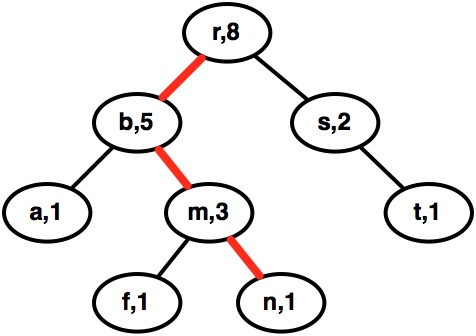
\includegraphics[width=2.5in]{binary-search-trees/rankSelect}
\end{center}
\end{example}


\begin{question}
  But how can we maintain the sizes of the subtrees as we perform
  various operations on the BST such as possibly aggregate insertions,
  deletions, splits, and joins?
\end{question}
%
To implement a size-augmented tree, we need to keep \cd{size} field at
each node and compute the size of the nodes as they are created.
%
In our parametric implementation, we can incorporate the \cd{size}
field by changing the definition of a node and initializing it to $1$,
when a singleton tree is created. 
%
When \cd{split} and \cd{join} functions create a new node, they
can compute its size by summing the sizes of its children.
%

In addition to the \texttt{rank} and \texttt{select} functions, we can
also define the function $\cd{splitRank}(T,i)$, which splits the
tree into two by returning the trees $t_1$ and $t_2$ such that $t_1$
contains all keys with rank less than $i$ and $t_2$ contains all keys
with rank is greater or equal to $i$. 
%
Such a function can be used for example to write divide-and-conquer
algorithms on imperfectly balanced trees.


% The implementation of \cd{splitRank} is similar to \cd{split}
% except when deciding which branch to take, we base it on the sizes
% instead of the keys.  Note that with \cd{splitRank} we can also
% implement \cd{select} as a \cd{splitRank} followed by a simple
% search for the first key of the second tree returned by
% \cd{splitRank}.



\subsection{Augmenting with Reduced Values}

To compute rank-based properties of keys in a BST, we augmented the
BST so that each node stores the size of its subtree.  More generally,
we might want to associate with each node a \defn{reduced value} that
is computed by reducing over the subtree rooted at the node by a user
specified function.  In general, there is no restriction on how the
reduced values may be computed, they can be based on keys or
additional values that the tree is augmented with.
%
To compute reduced values, we simply store with every node $u$ of a
binary search tree, the reduced value of its subtree (i.e. the sum of
all the reduced values that are descendants of $u$, possibly also the
value at $u$ itself).

\begin{example}
  The following drawing shows a tree with key-value pairs on the left,
  and the augmented tree on the right, where each node additionally
  maintains the sum of it subtree.
\begin{center}
  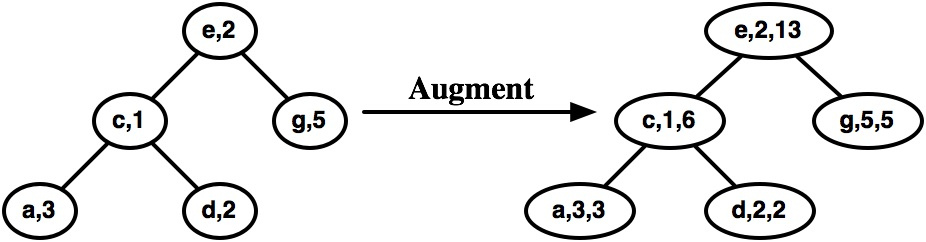
\includegraphics[width=4in]{binary-search-trees/augtree}
\end{center}
The sum at the root ($13$) is the sum of all values in the tree ($3 +
1 + 2 + 2 + 5$).    It is also the sum of the reduced values of its
two children ($6$ and $5$) and its own value $2$.
\end{example}



\input{binary-search-trees/fig-treaps-rvals}



The value of each reduced value in a tree can be calculated as the sum
of its two children plus the value stored at the node.  This means
that we can maintain these reduced values by simply taking the
``sum'' of three values whenever creating a node.  We can thus change
a data structure to support reduced values by changing the way we
create nodes.  In such a data structure, if the function that we use
for reduction performs constant work, then the work and the span bound
for the data structure remains unaffected.

As an example, \figref{bst::reducedjoin} describes an extension of the
parametric implementation of Treaps to support reduced values.  The
description is parametric in the values paired with keys and the
function \cd{f} used for reduction.  
%
The type for Treaps is extended to store the value paired with the key
as well as the reduced value.  Specifically, in a \cd{Node}, the
first data entry is the value paired by the key and the second is the
reduced value.
%


To compute reduced values as the structure of the tree changes, the
implementation relies on an auxiliary function \cd{mkNode} (read
``make node'') that takes the key-value pair as well as the left and
right subtrees and computes the reduced value by applying reducer
function to the values of the left and right subtrees as well as the
value.
%
The only difference in the implementation of \cd{split} and
\cd{join} functions from \chref{bst} is the use of \cd{mkNode}
instead of \cd{Node}.  

\begin{example}
The following diagram shows an example of splitting an augmented tree.
\begin{center}
  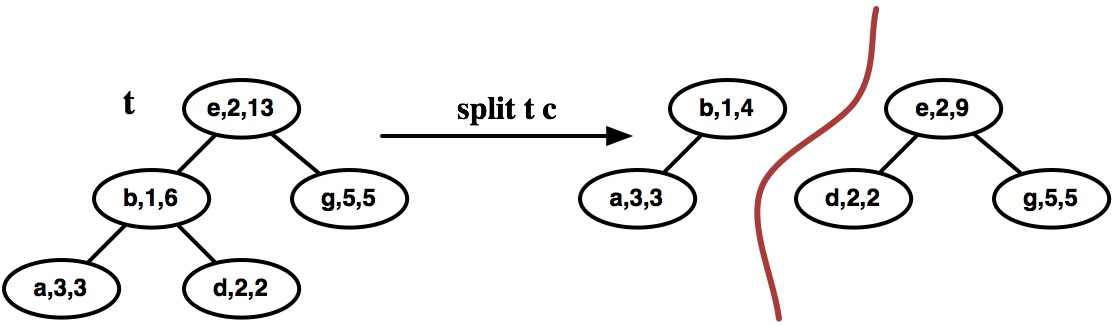
\includegraphics[width=5in]{binary-search-trees/augtree-split}
\end{center}
The tree is split by the key $c$, and the reduced values on the
internal nodes need to be updated.  This only needs to happen along
the path that created the split, which in this case is $e$, $b$, and
$d$.  The node for $d$ does not have to be updated since it is a leaf.
The \cd{makeNode} for $e$ and $b$ are what will update the reduced
values for those nodes.
\end{example}

We note that this idea can be used with any binary search tree, not
just Treaps.  We only need to replace the function for creating a node
so that as it creates the node, it also computes a reduced value for
the node by summing the reduced values of the children and the value
of the node itself.

\begin{remark}
  In an imperative implementation of binary search trees, when a child
  node is side affected, the reduced values for the nodes on the path
  from the modified node to the root must be recomputed.
\end{remark}

\section{Problems}

\begin{probl}{}
There are 18 subgraphs for a triangle consisting of three vertices
and three edges connecting them, including the empty graph and the graph
itself.    List them all.
\end{probl}


\begin{probl}{}
In star contraction, what is the probability that a vertex with degree
$d$ is removed.
\end{probl}


\begin{probl}{}
Find an example graph, where star-based graph contraction removes a
small number of edges on each round.
\end{probl}

% Solution: a graph consisting of small stars that are connected with
% many edges. The star will be removed but all the cross edges between
% them will remain.  Must repeat this recursively to find the right
% structure.

\begin{probl}{}
Describe how to construct a graph that exhibits the worst-case
behavior for \thmref{gc::star-contraction-cost}.
\end{probl}

\begin{probl}{}
Is the star contraction algorithm work-optimal for a dense graph with
$\Omega(n^2)$ edges? Prove or disprove.
\end{probl}



%% \section{Leftover material}

%% \section{Red-Black Trees}

%% \textbf{This is an early version.}
%% Another common near-balance scheme, used in many libraries, is the
%% red-black scheme.  The idea behind the scheme is to assign one of two
%% colors to each internal node of a BST.

%% \newcommand{\bh}{\overline{h}}
%% \begin{definition}[Red-Black Tree]
%% A red-black tree is a binary search tree $T$ along with a mapping from
%% every node to either \emph{black} or \emph{red} that satisfies the
%% following properties:
%% \begin{enumerate}
%% \item 
%% The root and all leaves are black.
%% \item
%% Every path from a node to a leaf contains the same number of black
%% nodes.
%% \item
%% A red node cannot have another red node as a parent.
%% \end{enumerate}
%% We define the \emph{black height} of a tree to be the number of black
%% nodes on the path to a leaf, and denote it as $\bh(t)$.
%% \end{definition}
%% The red-back tree properties guarantee that all leaves have a depth
%% that is within a factor of two of each other.      This is because
%% all paths to the leaves have the same number of black nodes, and the number
%% of red nodes in a path can be at most as many as black nodes.
%% Since all leaves are within a factor of two in depth,
%% the red-black trees have height $O(\lg |T|)$.   
%% \begin{exercise}
%% Prove that if in a binary tree $T$ all leaves have depth within a constant
%% factor of each other, then the tree has height $O(\lg |T|)$.
%% \end{exercise}

%% \begin{figure}
%% \begin{datastructure}[Implementing \adt{balancedBST} with red-black trees]~
%% \label{ds:redblack}
%% \begin{lstlisting}
%% datatype $\ccc$ = R | B@\vspace{.1in}@
%% datatype $\tttt$ = Leaf | iNode of ($\ccc$ ** $\tyint$ ** $\tttt$ ** $\kkk$ ** $\tttt$)@\vspace{.1in}@
%% val empty = Leaf@\vspace{.1in}@
%% fun singleton$(k)$ = Node(B,$1$,Leaf,$k$,Leaf)@\vspace{.1in}@
%% fun expose(Leaf) = Leaf
%%   | expose(iNode(_,_,$L,k,R$) => Node$(L,k,R)$@\vspace{.1in}@
%% fun $\bh(T)$ = case $T$ of 
%%             Leaf => 1
%%           | iNode(_,$h$,_,_,_) => $h$@\vspace{.1in}@
%% fun $c(T)$ = case $T$ of 
%%             Leaf => B
%%           | iNode($c$,_,_,_,_) => $c$@\vspace{.1in}@
%% fun blacken(iNode(R,$h,L,k,R$)) = iNode(B,$h+1,L,k,R$))
%%   | blacken($T$) = $T$@\vspace{.1in}@
%% fun joinLeft$(t_1,k,t_2)$ =      requires: $\bh(t_1) \leq \bh(t_2)$
%%   if $(\bh(t_1) = \bh(t_2)) \wedge (c(t_2) = \cd{B})$
%%   then iNode(R,$\bh(t_1),t_1,k,t_2$)
%%   else let 
%%       val iNode$(c_2,h_2,L_2,k_2,R_2)$ = $t_2$
%%       val ($T$ as iNode$(c_1,h_1,L_1,k_1,R_1))$ = joinLeft$(t_1,k,L_2)$
%%     in case $(c_1,c_2,h_1 = h_2)$ of
%%        (R,R,_)    => iNode$($B$,h_2+1,T,k_2,R_2)$
%%      | (B,B,true) => iNode$($R$,h_2,\cd{blacken}(L_1),k_1,\cd{iNode}($B$,h_2,R_1,k_2,R_2))$@\label{line:rbrotate}@
%%      |  _       => iNode$(c_2,h_2,T,k_2,R_2)$
%%     end@\vspace{.1in}@
%% fun joinMid$(t_1,k,t_2)$ =
%%   case compare$(\bh(t_1), \bh(t_2))$ of
%%      Less => blacken(joinLeft$(t_1,k,t_2)$)
%%      Equal => iNode(B,$\bh(t_1)+1,t_1,k,t_2$)
%%      Greater => blacken(joinRight$(t_1,k,t_2)$)
%% \end{lstlisting}
%% THIS CODE NOT DOUBLE CHECKED
%% \end{datastructure}
%% \end{figure}

%% \begin{comment}
%% Another version of joinLeft---much longer
%% \begin{lstlisting}
%% fun joinLeft$(t_1,k,t_2)$ =      requires: $h(t_1) \leq h(t_2)$
%%   if $h(t_1) = h(t_2)$
%%   then Node(R,$h(t_1),t_1,k,t_2$)
%%   else let 
%%       val Node$(c_2,h_2,L_2,k_2,R_2)$ = $t_2$
%%        in case $c(L_2)$ of
%%          R => (case joinLeftR$(t_1,k,L_2)$ of
%%                  Node(B,$h_1,L_1,k_1,R_1)$ =>
%%                    Node$($R$,h_2,\cd{blacken}(L_1),k_1,\cd{Node}($B$,h_2,R_1,k_2,R_2))$@\label{line:rbrotate}@
%%                | $T$ => Node$($B$,h_2,T,k_2,R_2)$)
%%         | B => NODE(B,$h_2,\cd{joinLeft}(t_1,k,L_2),k_2,R_2$)
%% and joinLeftR$(t_1,k,t_2)$ =
%%   let val Node$(c_2,h_2,L_2,k_2,R_2)$ = $t_2$
%%   in let val $T$ = joinLeft$(t_1,k,L_2)$
%%      in case $c(T)$ of
%%        R => Node$($B$,h_2+1,T,k_2,R_2)$
%%      | B => Node$($R$,h_2,T,k_2,R_2)$@\vspace{.1in}@
%% \end{lstlisting}
%% \end{comment}

%% Data Structure~\ref{ds:redblack} gives an implementation of
%% \adt{balancedBST} based on red-black trees.  As usual, all we need to
%% do is implement \cd{joinMid} so that when given two trees that
%% satisfy the red-black properties, it returns a tree that satisfy same
%% properties.    When joining trees $t_1$ and $t_2$, if they have the same
%% black height, we can just create a black node with those two trees as
%% children and $k$ as the key, and we are done.  However, if one tree is
%% higher than the other, then we have to rebalance in some way.  Let us
%% assume that $\bh(t_1) < \bh(t_2)$.  In the algorithm, the function
%% \cd{joinLeft} handles this case.  It basically searches down the
%% left spine of $t_2$ until it finds a black-rooted subtree $T'$ of the
%% same black height as $t_1$.  It then creates a red node containing
%% $t_1$, $k$, and $T'$.  This might violate the red property, which then
%% gets fixed on the way back up the recursion.

%% \begin{theorem}
%% For two red-black trees $t_1$ and $t_2$ and a key $k$ such that
%% $K(t_1) < k < K(t_2)$, \cd{joinMid}$(t_1,k,t_2)$ returns a
%% red-black tree containing $K(t_1) \cup \{k\} \cup K(t_2)$, and a black
%% root.
%% \end{theorem}
%% \begin{proof}
%% We just state the invariants for \cd{joinLeft}$(t_1,k,t_2)$.  The
%% function require the following conditions on its inputs: $\bh(t_1)
%% \leq \bh(t_2)$, $K(t_1) < k < K(t_2)$, both $t_1$ and $t_2$ have the
%% red-black properties, and the root of $t_1$ is black.  Given those
%% conditions it returns a tree $t_r$ with the red-black properties, and
%% the following additional properties: $\bh(t_2) \leq \bh(t_r) \leq
%% \bh(t_2) + 1$, and if $\bh(t_r) = \bh(t_2) + 1$ then the root of $t_r$
%% is black and its left child is red.
%% \end{proof}

%% \newcommand{\rrr}{\mathbb{R}}
%% %\newcommand{\rempty}{E}
%% %\newcommand{\rnode}{N}
%% \begin{comment}
%% datatype $\tttt$ = Leaf | Node of ($\tttt$ ** $\kkk$ ** $\tttt$)@\vspace{.1in}@
%% \end{comment}




%% \section{AVL Trees}

%% \textbf{This section currently only contains the code.}

%% \begin{figure}
%% \begin{datastructure}[Implementing \adt{balancedBST} with AVL trees]~
%% \begin{lstlisting}
%% datatype $\tttt$ = Leaf | iNode of ($\tyint$ ** $\tttt$ ** $\kkk$ ** $\tttt$)@\vspace{.1in}@
%% val empty = Leaf@\vspace{.1in}@
%% fun singleton$(k)$ = Node($1$,Leaf,$k$,Leaf)@\vspace{.1in}@
%% fun expose(Leaf) = Leaf
%%   | expose(iNode(_,$L,k,R$) => Node$(L,k,R)$@\vspace{.1in}@
%% fun $h(T)$ = case $T$ of 
%%             Leaf => 0
%%           | iNode($h$,_,_,_) => $h$@\vspace{.1in}@
%% fun newNode$(t_1,k,t_2)$ =
%%    iNode$(1+ \max(h(t_1),h(t_2)),t_1,k,t_2)$@\vspace{.1in}@
%% fun rotateRight$(t_1\cd{ as iNode}(h_1,L_1,k_1,R_1), k, t_2$) =
%%   if $h_1 > h(t_2) + 1$ 
%%   then iNode$(h_1,L_1,k_1,\cd{iNode}(h_1-1,R_1,k,t_2))$
%%   else newNode$(t_1,k,t_2)$@\vspace{.1in}@
%% fun joinLeft$(t_1,k,t_2)$ =
%%   if $h(t_1) \geq h(t_2)$ 
%%   then newNode$(t_1,k,t_2)$
%%   else let val iNode$(h_2,L_2,k_2,R_2)$ = $t_2$
%%      in rotateRight$(\cd{joinLeft}(t_1,k,L_2),k_2,t_2)$ end@\vspace{.1in}@
%% fun joinMid$(t_1,k,t_2)$ =
%%   if $h(t_1) < h(t_2) - 1$ then joinLeft$(t_1,k,t_2)$
%%   else if $h(t_2) < h(t_1) - 1$ then joinRight$(t_1,k,t_2)$
%%   else newNode$(t_1,k,t_2)$@\vspace{.1in}@
%% \end{lstlisting}
%% THIS CODE NOT DOUBLE CHECKED
%% \begin{comment}
%% Not including the following since it is redundant.
%% removeMin and join are common among implementations.
%% joinRight is by symmetry
%% \begin{lstlisting}
%% fun rotateLeft$(t_1,k,t_2 \cd{ as Node}(h_2,L_2,k_2,R_2))$ =
%%   if $h_2 > h(t_1) + 1$ 
%%   then Node$(h_2,\cd{Node}(h_2-1,t_1,k,L_2),k_2,R_2)$
%%   else newNode$(t_1,k,t_2)$@\vspace{.1in}@
%% fun joinRight$(t_1,k,t_2)$ =
%%   if $h(t_2) \geq h(t_1)$ then newNode$(t_1,k,t_2)$
%%   else let val Node$(h_1,L_1,k_1,R_1)$ = $t_1$
%%      in rotateLeft$(L_1,k_1,\cd{joinRight}(R_1,k,t_2))$ end@\vspace{.1in}@
%% fun removeMin$(T)$ =
%%   case $T$ of
%%     Node$(\_,\cd{Leaf},k,\_)$ => $(k,R)$
%%   | Node$(\_,L,k,R)$ =>
%%       let val $(m,L')$ = removeMin$(L)$
%%       in $(m,\cd{rotateLeft}(L',k,R))$ end@\vspace{.1in}@
%% fun join$(t_1,m,t_2)$ =
%%   case ($m$,$t_2$) of
%%     (Some(k),_) => joinMid$(t_1,k,t_2)$
%%   | (None,Leaf) => $t_1$
%%   | (None,_) => 
%%       let val $(k,t_2')$ = removeMin$(t_2)$
%%       in joinMid$(t_1,k,t_2')$ end
%% \end{lstlisting}
%% \end{comment}
%% \end{datastructure}
%% \end{figure}

%% \paragraph{No Balancing.}

%% \begin{figure}
%% \begin{datastructure}[Implementing \adt{balancedBST} with no balance criteria]~
%% \label{ds:bstjoin}
%% \begin{lstlisting}
%% datatype $\tttt$ = Leaf | Node of ($\tttt$ ** $\kkk$ ** $\tttt$)@
%% \vspace{.1in}@
%% val empty = Leaf@
%% \vspace{.1in}@
%% function singleton$(k)$ = Node(Leaf,$k$,Leaf)@
%% \vspace{.1in}@
%% function expose$(T)$ = $T$@
%% \vspace{.1in}@
%% function split$(T,k)$ =
%%   case expose$(T)$ of
%%     Leaf => (Leaf, False, Leaf)
%%   | Node$(L,k',R)$ =
%%       case compare$(k,k')$ of
%%         LESS => @\label{line:split-less}@
%%           let val $(L',m',R')$ = split$(L,k)$
%%           in $(L',m',\cd{Node}(R',k',R))$ end @\label{line:splitnode1}@
%%       | EQUAL => $(L,~\cd{True},R)$
%%       | GREATER => @\label{line:split-greater}@
%%           let val $(L',m',R')$ = split$(R,k)$
%%           in (Node$(L,k',L'),m',R'$) end @\label{line:splitnode2}@@
%% \vspace{.1in}@
%% function join$(t_1,m,t_2)$ =
%%   case $m$ of
%%     Some$(k)$ => Node$(t_1,k,t_2)$
%%   | None =>
%%       case $t_1$ of
%%         Leaf => $t_2$
%%       | Node$(L,k,R)$ => Node$(L,k,~\cd{join}(R,\cnone,t_2)))$@
%% \end{lstlisting}
%% \end{datastructure}
%% \end{figure}

%% \paragraph{BSTs without balance.}
%% If we do not care about balance, then the BST interface is reasonably easy
%% to implement, and is given in Data Structure~\ref{ds:bstjoin}.    
%% The \cd{split} algorithm recursively traverses the tree from the
%% root to the key $k$ splitting along the path, and then when returning from
%% the recursive calls, it puts the subtrees back together.
%% \begin{example}
%% In the following tree we split on the key $c$, which does not appear
%% in the tree.  The split traverses
%% the path $\cseq{a,e,b,d}$ turning right at $a$ and $b$
%% (line~\ref{line:split-greater} of the Data Structure~\ref{ds:bstjoin})
%% and turning left at $e$ and $d$ (line~\ref{line:split-less}).  The
%% pieces are put back together into the two resulting trees on the way
%% back up the recursion.  
%% \begin{center}
%%   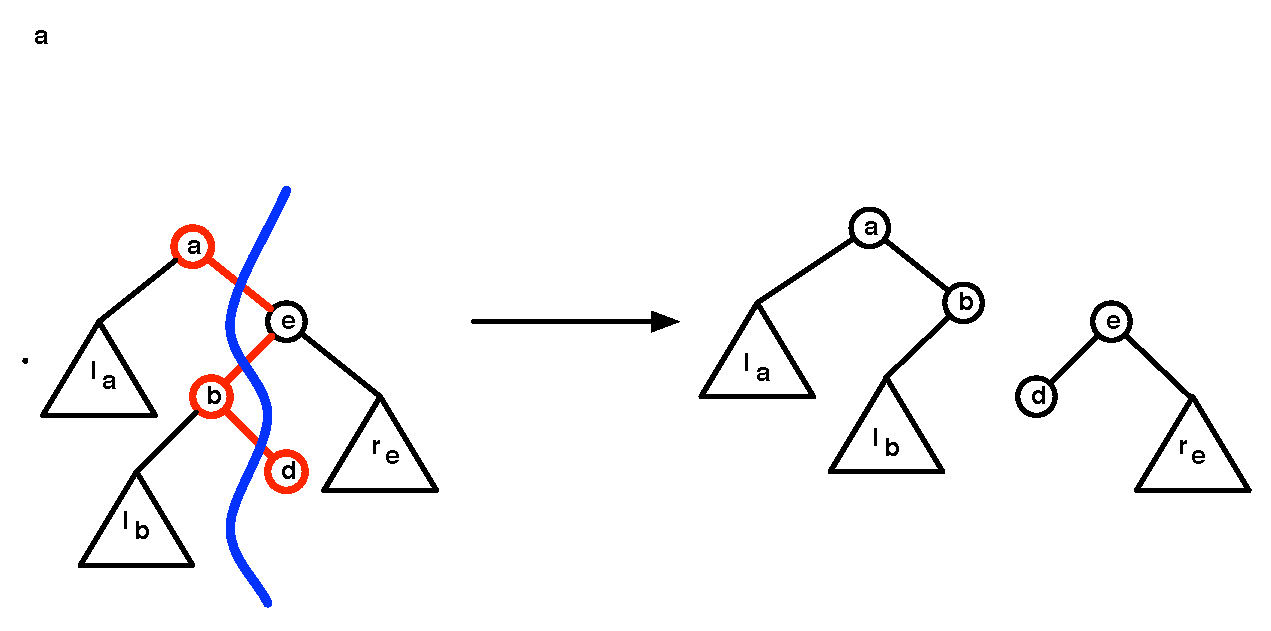
\includegraphics[width=5.7in]{binary-search-trees/bstsplit}
%% \end{center}
%% %The actual way the trees will be put back together will depend on the
%% %balancing scheme.
%% \end{example}
%% The \cd{join} algorithm with a key in the middle simply calls
%% \cd{Node} and therefore does constant work.  For near-balanced
%% trees, however, \cd{join} needs to rebalance the tree and can take
%% work proportional to the height of the trees.

%% \begin{example}
%% Using the version of \cd{join} with no rebalancing (from Data Structure~\ref{ds:bstjoin})
%% we have:
%% \[\cd{join}\left(
%% \raisebox{-.45in}{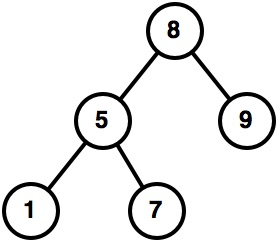
\includegraphics[scale=.6]{binary-search-trees/bst4}}~~,
%% ~\cd{Some}(10)~,
%% ~\cd{Leaf}
%% \right) \Rightarrow 
%% \raisebox{-.7in}{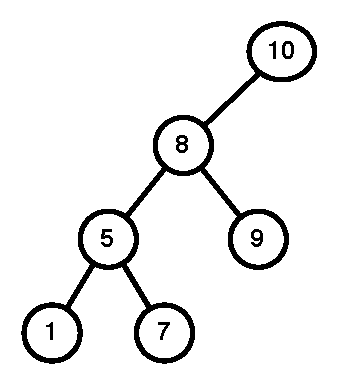
\includegraphics[scale=.6]{binary-search-trees/bst4d}}
%% \]
%% The resulting tree is clearly not balanced since we joined a tree of
%% height three with one of height zero and did no rebalancing.  The join
%% in a near-balanced scheme needs to rebalance the tree, as we will see
%% later.
%% \end{example}

%% \paragraph{Minimal Interface.}
%% We refer to a join that always takes a key in the middle
%% \cd{joinMid}$(L,k,R)$ and one that never takes a key as
%% \cd{joinPair}$(L,R)$.  It turns out that we only need one of these
%% and the other can be efficiently implemented using it.  For
%% example:
%% \begin{lstlisting}[numbers=none]
%% joinMid$(L,k,R)$ = joinPair($L$,joinPair(singleton($k$),R)
%% \end{lstlisting}
%% \begin{exercise}
%% Implement \cd{joinPair} with \cd{joinMid} and any other
%% functions in the balancedBST ADT.
%% \end{exercise}
%% It is also possible to implement \cd{split} efficiently with
%% \cd{join}.  Indeed the algorithm for such a split is the same code
%% as in Data Structure~\ref{ds:bstjoin}, except that the
%% \cd{Node} on Lines~\ref{line:splitnode1} and~\ref{line:splitnode2}
%% replaced with \cd{joinMid}.
%% This implies that to achieve a new asymptotically efficient
%% implementation of a near balanced BST scheme, all one needs to
%% implement is one of \cd{joinMid} or \cd{joinPair}, along with
%% supplying \cd{expose} and \cd{empty} (\cd{singleton}$(k)$ is
%% easily defined as \cd{joinMid(empty,$k$,empty)}).  

%% \begin{comment}
%% \begin{exercise}
%% Write a version of \cd{insert} that takes a function $f : \data
%% \times \data$ and if the insertion key $k$ is already in the tree
%% applies $f$ to the old and new value to return the value to associate
%% with the key.
%% \end{exercise}
%% \end{comment}



\begin{comment}

Consider now a call to \cd{union} with parameters
$t_1$ and $t_2$.  To simplify the analysis, we will make the following
assumptions:
\begin{enumerate}
\item $t_1$ it is perfectly balanced (i.e., \cexpose{} returns subtrees of
  size at most $|t_1|/2$), 
\item each time a key from $t_1$ splits $t_2$, it splits the tree in
  exactly in half, and
\item without loss of generality let $|t_1| \leq |t_2|$.
\end{enumerate}
Later we will relax these assumptions.  Let us define $m = |t_1|$ and
$n = |t_2|$ (recall the size of a tree is the number of keys in it).
With these assumptions and examining the algorithm we can then write
the following recurrence for the work of \cd{union}:
\begin{align*}
  W_{\mbox{union}}(m, n) &\leq 2W_{\mbox{union}}(m/2,n/2) + W_{\mbox{split}}(n)
+ W_{\mbox{join}}(n+m) + O(1)\\
   & \leq  2W_{\mbox{union}}(m/2, n/2) + O(\lg n)~.
\end{align*}  
The size for join is the sum of the two sizes, $m+n$, but since 
$m \leq n$, $O(\lg (n + m))$ is equivalent to $O(\lg n)$.
We also have the base case
\begin{align*}
  W_{\mbox{union}}(1, n) & \leq 2W_{\mbox{union}}(0,n/2) + W_{\mbox{split}}(n)
+ W_{\mbox{join}}(n) + O(1)\\
         & \leq O(\lg n)~.
\end{align*}
The final inequality is since $2W_{\mbox{union}}(0,n) = O(1)$.

We can draw the recursion tree showing the work performed by the
splitting of $t_2$ and by the joining of the results as follows.

%This figure should be changed so "n" is replaced by "N" except the
%bottom level should be "each costs log (1 + n/m)"

\begin{center}
  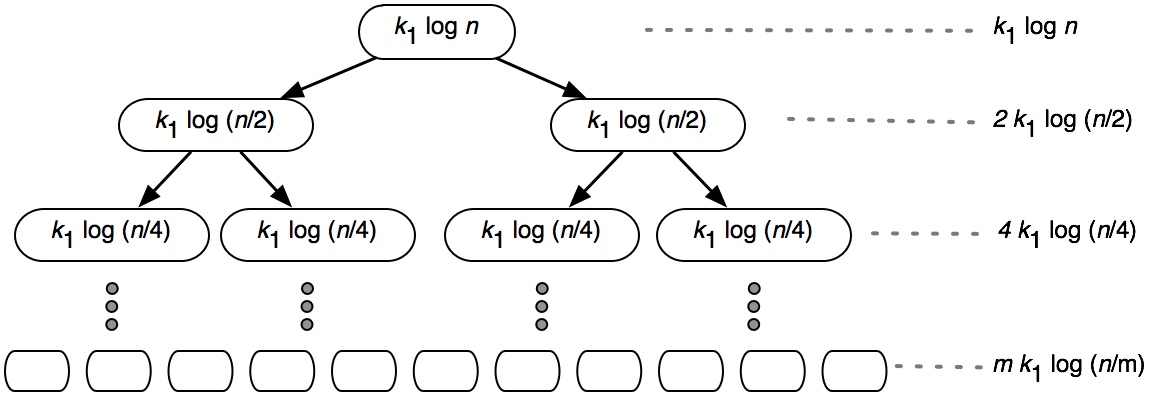
\includegraphics[scale=.65]{binary-search-trees/recurtree2}
\end{center}
%



There are several features of this tree that's worth mentioning:
First, ignoring the somewhat-peculiar cost in the base case, we know
that this tree is leaf-dominated.  Therefore, excluding the cost at
the bottom level, the cost of \cunion{} is $O(\#\text{ of leaves})$
times the cost of each leaf.

\begin{question}
How many leaves are there?
\end{question}
%
To find the number of leaves, let's take a closer look at the work
recurrence.  Notice that in the recurrence, the tree bottoms out when
$m = 1$ and before that, $m$ always gets split in half (remember that
$t_1$ is perfectly balanced).  The tree $t_2$ does not affects the
shape of the recursion tree or the stopping condition.  Therefore,
this is yet another recurrence of the form $f(m) = 2f(m/2) + O(...)$,
which means that there are $m$ leaves.
%
\begin{question}
How deep are the leaves?
\end{question}
%
By the same reasoning, we can see that the leaves are $(1 + \lg m)$
deep.

Let's now determine the size of $t_2$ at the leaves.  
%
We have $m$ keys in $t_1$ to start with, and they split $t_2$ evenly
(by assumption), thus, the leaves have all the same size of
$\frac{n}{m}$.
%
Therefore, each leaf costs $O(\lg (1+\frac{n}{m}))$ (the $1+$ is
needed to deal with the case that $n = m$).  Since there are $m$
leaves, the whole bottom level costs $O(m \lg (1+ \frac{n}{m}))$.
Hence, if the trees satisfy our assumptions, we have that \cunion{}
runs in $ O( m\lg(1 + \frac{n}{m}))$ work.

%\paragraph{Removing An Assumption:}

Of course, in reality, our keys in $t_1$ won't split subtrees of $t_2$
in half every time.  But it turns out that any unevenness in the
splitting only helps reduce the work---i.e., the perfect split is the
worst case.  We won't go through a rigorous argument, but if we keep
the assumption that $t_1$ is perfectly balanced, then the shape of the
recursion tree stays the same.  What is now different is the cost at
each level.  Let us try to analyze the cost at level $i$.  At this
level, there are $k = 2^i$ nodes in the recursion tree. Say the sizes
of $t_2$ at these nodes are $n_1, \dots, n_k$, where $\sum_j n_j =
n$. Then, the total cost for this level is
\[
c \cdot \sum_{j=1}^k \lg (n_j) \;\;\leq\;\; c \cdot \sum_{j=1}^k \lg (n/k) =
c\cdot 2^i \cdot \lg (n/2^i),
\]
where we used the fact that the logarithm function is
concave\footnote{Technically, we're applying the so-called Jensen's
  inequality.}.  Thus, the tree remains leaf-dominated and the same
reasoning shows that the total work is $O(m \lg (1 + \frac{n}{m}))$.

Still, in reality, $t_1$ doesn't have to be perfectly balanced as we
assumed. A similar reasoning can be used to show that $t_1$ only has
to be approximately balanced. We will leave this case as an exercise.

We end by remarking that as described, the span of \cunion{} is
$O(\lg^2 n)$, but this can be improved to $O(\lg n)$ by changing the
algorithm slightly.

In summary, \cunion{} can be implemented in $O(m \lg (1 +
\tfrac{n}m))$ work and span $O(\lg n)$.  

Essentially the same analysis applies to the functions
\cd{intersection} and \cd{difference}, whose structures are the same
as \cd{union}, except for an additional constant work and span for
the conditional (\cd{if}) expression.

\end{comment}

\flushchapter





